\chapter{Connectedness and Compactness}

In the study of calculus, there are three basic theorems about continuous functions, and on these theorems the rest of calculus depends. They are the following:

Intermediate value theorem. If \(f: \left\lbrack {a,b}\right\rbrack \rightarrow \mathbb{R}\) is continuous and if \(r\) is a real number between \(f\left( a\right)\) and \(f\left( b\right)\) , then there exists an element \(c \in \left\lbrack {a,b}\right\rbrack\) such that \(f\left( c\right) = r\) .

Maximum value theorem. If \(f: \left\lbrack {a,b}\right\rbrack \rightarrow R\) is continuous, then there exists an element \(c \in \left\lbrack {a,b}\right\rbrack\) such that \(f\left( x\right) \leq f\left( c\right)\) for every \(x \in \left\lbrack {a,b}\right\rbrack\) .

Uniform continuity theorem. If \(f: \left\lbrack {a,b}\right\rbrack \rightarrow \mathbb{R}\) is continuous, then given \(\epsilon > 0\) , there exists \(\delta > 0\) such that \(\left| {f\left( {x}_{1}\right) - f\left( {x}_{2}\right) }\right| < \epsilon\) for every pair of numbers \({x}_{1},{x}_{2}\) of \(\left\lbrack {a,b}\right\rbrack\) for which \(\left| {{x}_{1} - {x}_{2}}\right| < \delta\) .

These theorems are used in a number of places. The intermediate value theorem is used for instance in constructing inverse functions, such as \(\sqrt[3]{x}\) and arcsin \(x\) ; and the maximum value theorem is used for proving the mean value theorem for derivatives, upon which the two fundamental theorems of calculus depend. The uniform continuity theorem is used, among other things, for proving that every continuous function is integrable.

We have spoken of these three theorems as theorems about continuous functions. But they can also be considered as theorems about the closed interval \(\left\lbrack {a,b}\right\rbrack\) of real numbers. The theorems depend not only on the continuity of \(f\) but also on properties of the topological space \(\left\lbrack {a,b}\right\rbrack\) .

The property of the space \(\left\lbrack {a,b}\right\rbrack\) on which the intermediate value theorem depends is the property called connectedness, and the property on which the other two depend is the property called compactness. In this chapter, we shall define these properties for arbitrary topological spaces, and shall prove the appropriate generalized versions of these theorems.

As the three quoted theorems are fundamental for the theory of calculus, so are the notions of connectedness and compactness fundamental in higher analysis, geometry, and topology-indeed, in almost any subject for which the notion of topological space itself is relevant.

\section*{§ 23 Connected Spaces}

The definition of connectedness for a topological space is a quite natural one. One says that a space can be ``separated'' if it can be broken up into two ``globs''—disjoint open sets. Otherwise, one says that it is connected. From this simple idea much follows.

\begin{definition} Let \(X\) be a topological space. A separation of \(X\) is a pair \(U,V\) of disjoint nonempty open subsets of \(X\) whose union is \(X\) . The space \(X\) is said to be connected if there does not exist a separation of \(X\) .
\end{definition}


Connectedness is obviously a topological property, since it is formulated entirely in terms of the collection of open sets of \(X\) . Said differently, if \(X\) is connected, so is any space homeomorphic to \(X\) .

Another way of formulating the definition of connectedness is the following:

A space \(X\) is connected if and only if the only subsets of \(X\) that are both open and closed in \(X\) are the empty set and \(X\) itself.

For if \(A\) is a nonempty proper subset of \(X\) that is both open and closed in \(X\) , then the sets \(U = A\) and \(V = X - A\) constitute a separation of \(X\) , for they are open, disjoint, and nonempty, and their union is \(X\) . Conversely, if \(U\) and \(V\) form a separation of \(X\) , then \(U\) is nonempty and different from \(X\) , and it is both open and closed in \(X\) .

For a subspace \(Y\) of a topological space \(X\) , there is another useful way of formulating the definition of connectedness:

\begin{lemma} If \(Y\) is a subspace of \(X\) , a separation of \(Y\) is a pair of disjoint nonempty sets \(A\) and \(B\) whose union is \(Y\) , neither of which contains a limit point of the other. The space \(Y\) is connected if there exists no separation of \(Y\) .
\end{lemma}

\begin{proof}
Suppose first that \(A\) and \(B\) form a separation of \(Y\) . Then \(A\) is both open and closed in \(Y\) . The closure of \(A\) in \(Y\) is the set \(\bar{A} \cap Y\) (where \(\bar{A}\) as usual denotes the closure of \(A\) in \(X\) ). Since \(A\) is closed in \(Y,A = \bar{A} \cap Y\) ; or to say the same thing, \(\bar{A} \cap B = \varnothing\) . Since \(A\) is the union of \(A\) and its limit points, \(B\) contains no limit points of \(A\) . A similar argument shows that \(A\) contains no limit points of \(B\) .

Conversely, suppose that \(A\) and \(B\) are disjoint nonempty sets whose union is \(Y\) , neither of which contains a limit point of the other. Then \(\bar{A} \cap B = \varnothing\) and \(A \cap \bar{B} = \varnothing\) ; therefore, we conclude that \(\bar{A} \cap Y = A\) and \(\bar{B} \cap Y = B\) . Thus both \(A\) and \(B\) are closed in \(Y\) , and since \(A = Y - B\) and \(B = Y - A\) , they are open in \(Y\) as well.
\end{proof}

\begin{centeredblock}
\begin{example} Let \(X\) denote a two-point space in the indiscrete topology. Obviously there is no separation of \(X\) , so \(X\) is connected.
\end{example}
\end{centeredblock}

\begin{centeredblock}
\begin{example} Let \(Y\) denote the subspace \(\left\lbrack {-1,0)\cup (0,1}\right\rbrack\) of the real line \(\mathbb{R}\) . Each of the sets \(\left\lbrack {-1,0)\text{ and }(0,1}\right\rbrack\) is nonempty and open in \(Y\) (although not in \(\mathbb{R}\) ); therefore, they form a separation of \(Y\) . Alternatively, note that neither of these sets contains a limit point of the other. (They do have a limit point 0 in common, but that does not matter.)
\end{example}
\end{centeredblock}

\begin{centeredblock}
\begin{example} Let \(X\) be the subspace \(\left\lbrack {-1,1}\right\rbrack\) of the real line. The sets \(\left\lbrack {-1,0}\right\rbrack\) and \((0,1\rbrack\) are disjoint and nonempty, but they do not form a separation of \(X\) , because the first set is not open in \(X\) . Alternatively, note that the first set contains a limit point,0, of the second. Indeed, there exists \(n\) o separation of the space \(\left\lbrack {-1,1}\right\rbrack\) . We shall prove this fact shortly
\end{example}
\end{centeredblock}

\begin{centeredblock}
\begin{example} The rationals \(\mathbb{Q}\) are not connected. Indeed, the only connected subspaces of \(\mathbb{Q}\) are the one-point sets \(\cdot\) If \(Y\) is a subspace of \(\mathbb{Q}\) containing two points \(p\) and \(q\) , one can choose an irrational number a lying between \(p\) and \(q\) , and write \(Y\) as the union of the open sets

\[
Y \cap \left( {-\infty,a}\right) \;\text{ and }\;Y \cap \left( {a, + \infty }\right) .
\]
\end{example}
\end{centeredblock}

\begin{centeredblock}
\begin{example} Consider the following subset of the plane \({\mathbb{R}}^{2}\) :

\[
X = \{ x \times y \mid y = 0\} \cup \{ x \times y \mid x > 0\text{ and }y = 1/x\} .
\]

Then \(X\) is not connected, indeed, the two indicated sets form a separation of \(X\) because neither contains a limit point of the other. See Figure 23.1.

\begin{center}
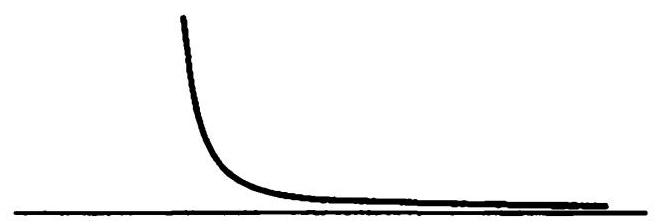
\includegraphics[width=0.6\textwidth]{images/23.1.jpg}
\end{center}
\hspace*{3em}

Figure 23.1
\end{example}
\end{centeredblock}

We have given several examples of spaces that are not connected. How can one construct spaces that are connected? We shall now prove several theorems that tell how to form new connected spaces from given ones. In the next section we shall apply these theorems to show that some specific spaces, such as intervals in \(\mathbb{R}\) , and balls and cubes in \({\mathbb{R}}^{n}\) , are connected. First, a lemma:

\begin{lemma} If the sets \(C\) and \(D\) form a separation of \(X\) , and if \(Y\) is a connected subspace of \(X\) , then \(Y\) lies entirely within either \(C\) or \(D\) .
\end{lemma}

\begin{proof}
Since \(C\) and \(D\) are both open in \(X\) , the sets \(C \cap Y\) and \(D \cap Y\) are open in \(Y\) . These two sets are disjoint and their union is \(Y\) ; if they were both nonempty, they would constitute a separation of \(Y\) . Therefore, one of them is empty. Hence \(Y\) must lie entirely in \(C\) or in \(D\)
\end{proof}

\begin{theorem} The union of a collection of connected subspaces of \(X\) that have a point in common is connected.

\end{theorem}
Proof. Let \(\left\{ {A}_{\alpha }\right\}\) be a collection of connected subspaces of a space \(X\) ; let \(p\) be a point of \(\bigcap {A}_{\alpha }\) . We prove that the space \(Y = \bigcup {A}_{\alpha }\) is connected. Suppose that \(Y = C \cup D\) is a separation of \(Y\) . The point \(p\) is in one of the sets \(C\) or \(D\) ; suppose \(p \in C\) . Since \({A}_{\alpha }\) is connected, it must lie entirely in either \(C\) or \(D\) , and it cannot lie in \(D\) because it contains the point \(p\) of \(C\) . Hence \({A}_{\alpha } \subset C\) for every \(\alpha\) , so that \(\bigcup {A}_{\alpha } \subset C\) , contradicting the fact that \(D\) is nonempty.

\begin{theorem} Let \(A\) be a connected subspace of \(X\) . If \(A \subset B \subset \bar{A}\) , then \(B\) is also connected.

Said differently: If \(B\) is formed by adjoining to the connected subspace \(A\) some or all of its limit points, then \(B\) is connected.

\end{theorem}
\begin{proof} Let \(A\) be connected and let \(A \subset B \subset \bar{A}\) . Suppose that \(B = C \cup D\) is a separation of \(B\) . By Lemma 23.2, the set \(A\) must lie entirely in \(C\) or in \(D\) ; suppose that \(A \subset C\) . Then \(\widetilde{A} \subset \widetilde{C}\) ; since \(\widetilde{C}\) and \(D\) are disjoint, \(B\) cannot intersect \(D\) . This contradicts the fact that \(D\) is a nonempty subset of \(B\) .
\end{proof}

\begin{theorem} The image of a connected space under a continuous map is connected.

\end{theorem}
\begin{proof} Let \(f: X \rightarrow Y\) be a continuous map; let \(X\) be connected. We wish to prove the image space \(Z = f\left( X\right)\) is connected. Since the map obtained from \(f\) by restricting its range to the space \(Z\) is also continuous, it suffices to consider the case of a continuous surjective map

\[
g: X \rightarrow Z\text{ . }
\]

Suppose that \(Z = A \cup B\) is a separation of \(Z\) into two disjoint nonempty sets open in \(Z\) . Then \({g}^{-1}\left( A\right)\) and \({g}^{-1}\left( B\right)\) are disjoint sets whose union is \(X\) ; they are open in \(X\) because \(g\) is continuous, and nonempty because \(g\) is surjective. Therefore, they form a separation of \(X\) , contradicting the assumption that \(X\) is connected.
\end{proof}

\section*{Theorem 23.6. A finite cartesian product of connected spaces is connected.}

\begin{proof}
We prove the theorem first for the product of two connected spaces \(X\) and \(Y\) . This proof is easy to visualize. Choose a ``base point'' \(a \times b\) in the product \(X \times Y\) . Note that the ``horizontal slice'' \(X \times b\) is connected, being homeomorphic with \(X\) , and each ``vertical slice'' \(x \times Y\) is connected, being homeomorphic with \(Y\) . As a result, each ``T-shaped'' space

\[
{T}_{x} = \left( {X \times b}\right) \cup \left( {x \times Y}\right)
\]

is connected, being the union of two connected spaces that have the point \(x \times b\) in common. See Figure 23.2. Now form the union \(\mathop{\bigcup }\limits_{{x \in X}}{T}_{x}\) of all these T-shaped spaces. This union is connected because it is the union of a collection of connected spaces that have the point \(a \times b\) in common. Since this union equals \(X \times Y\) , the space \(X \times Y\) is connected.

\begin{center}
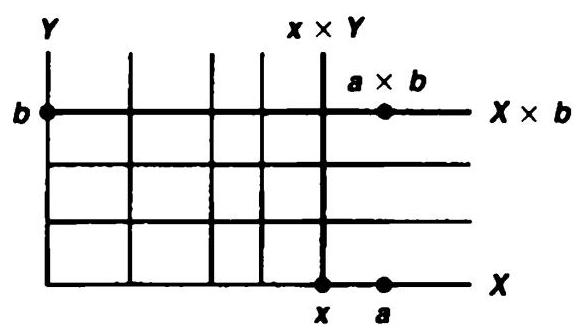
\includegraphics[width=0.5\textwidth]{images/23.2.jpg}
\end{center}
\hspace*{3em} 

Figure 23.2

The proof for any finite product of connected spaces follows by induction, using the fact (easily proved) that \({X}_{1} \times \cdots \times {X}_{n}\) is homeomorphic with \(\left( {{X}_{1} \times \cdots \times {X}_{n - 1}}\right) \times\) \({X}_{n}\) .

It is natural to ask whether this theorem extends to arbitrary products of connected spaces. The answer depends on which topology is used for the product, as the following examples show.
\end{proof}

\begin{centeredblock}
\begin{example} Consider the cartesian product \({\mathbb{R}}^{\omega }\) in the box topology. We can write \({\mathbb{R}}^{\omega }\) as the union of the set \(A\) consisting of all bounded sequences of real numbers, and the set \(B\) of all unbounded sequences. These sets are disjoint, and each is open in the box topology For if \(\mathbf{a}\) is a point of \({\mathbb{R}}^{\omega }\) , the open set

\[
U = \left( {{a}_{1} - 1,{a}_{1} + 1}\right) \times \left( {{a}_{2} - 1,{a}_{2} + 1}\right) \times
\]

consists enturely of bounded sequences if \(a\) is bounded, and of unbounded sequences if \(a\) if unbounded. Thus, even though \(\mathbb{R}\) is connected (as we shall prove in the next section), \({\mathbb{R}}^{\omega }\) is not connected in the box topology.
\end{example}
\end{centeredblock}

\begin{centeredblock}
\begin{example} Now consider \({\mathbb{R}}^{\omega }\) in the product topology. Assuming that \(\mathbb{R}\) is connected, we show that \({\mathbb{R}}^{\omega }\) is connected. Let \({\overline{\mathbb{R}}}^{n}\) denote the subspace of \({\mathbb{R}}^{\omega }\) consisting of all sequences \(\mathbf{x} = \left( {{x}_{1},{x}_{2},\ldots }\right)\) such that \({x}_{i} = 0\) for \(i > n\) The space \({\overline{\mathbb{R}}}^{n}\) is clearly homeomorphic to \({\mathbb{R}}^{n}\) , so that it is connected, by the preceding theorem. It follows that the space \({\mathbb{R}}^{\infty }\) that is the union of the spaces \({\overline{\mathbb{R}}}^{n}\) is connected, for these spaces have the point \(\mathbf{0} = \left( {0,0,\ldots }\right)\) in common. We show that the closure of \({\mathbb{R}}^{\infty }\) equals all of \({\mathbb{R}}^{\omega }\) , from which it follows that \({\mathbb{R}}^{\omega }\) is connected as well.

Let \(\mathbf{a} = \left( {{a}_{1},{a}_{2},\ldots }\right)\) be a point of \({\mathbb{R}}^{\omega }\) . Let \(U = \prod {U}_{i}\) be a basis element for the product topology that contains a. We show that \(U\) intersects \({\mathbb{R}}^{\infty }\) . There is an integer \(N\) such that \({U}_{i} = \mathbb{R}\) for \(i > N\) . Then the point

\[
\mathbf{x} = \left( {{a}_{1},\ldots,{a}_{n},0,0,\;}\right)
\]

of \({\mathbb{R}}^{\infty }\) belongs to \(U\) , since \({a}_{i} \in {U}_{i}\) for all \(i\) , and \(0 \in {U}_{i}\) for \(i > N\) .
\end{example}
\end{centeredblock}

The argument just given generalizes to show that an arbitrary product of connected spaces is connected in the product topology. Since we shall not need this result, we leave the proof to the exercises.

\section*{Exercises}

1. Let \(\mathcal{T}\) and \({\mathcal{T}}^{\prime }\) be two topologies on \(X\) . If \({\mathcal{T}}^{\prime } \supset \mathcal{T}\) , what does connectedness of \(X\) in one topology imply about connectedness in the other?

2. Let \(\left\{ {A}_{n}\right\}\) be a sequence of connected subspaces of \(X\) , such that \({A}_{n} \cap {A}_{n + 1} \neq \varnothing\) for all \(n\) . Show that \(\bigcup {A}_{n}\) is connected.

3. Let \(\left\{ {A}_{\alpha }\right\}\) be a collection of connected subspaces of \(X\) ; let \(A\) be a connected subspace of \(X\) . Show that if \(A \cap {A}_{\alpha } \neq \varnothing\) for all \(\alpha\) , then \(A \cup \left( {\bigcup {A}_{\alpha }}\right)\) is connected.

4. Show that if \(X\) is an infinite set, it is connected in the finite complement topology.

5. A space is totally disconnected if its only connected subspaces are one-point sets. Show that if \(X\) has the discrete topology, then \(X\) is totally disconnected. Does the converse hold?

6. Let \(A \subset X\) Show that if \(C\) is a connected subspace of \(X\) that intersects both \(A\) and \(X - A\) , then \(C\) intersects \(\operatorname{Bd}A\) .

7. Is the space \({\mathbb{R}}_{\ell }\) connected? Justify your answer.

8. Determine whether or not \({\mathbb{R}}^{\omega }\) is connected in the uniform topology.

9. Let \(A\) be a proper subset of \(X\) , and let \(B\) be a proper subset of \(Y\) . If \(X\) and \(Y\) are connected, show that

\[
\left( {X \times Y}\right) - \left( {A \times B}\right)
\]

is connected.

10. Let \({\left\{ {X}_{\alpha }\right\} }_{\alpha \in J}\) be an indexed family of connected spaces; let \(X\) be the product space

\[
X = \mathop{\prod }\limits_{{\alpha \in J}}{X}_{\alpha }
\]

Let \(\mathbf{a} = \left( {a}_{\alpha }\right)\) be a fixed point of \(X\) .

(a) Given any finite subset \(K\) of \(J\) , let \({X}_{K}\) denote the subspace of \(X\) consisting of all points \(\mathbf{x} = \left( {x}_{\alpha }\right)\) such that \({x}_{\alpha } = {a}_{\alpha }\) for \(\alpha \notin K\) . Show that \({X}_{K}\) is connected.

(b) Show that the union \(Y\) of the spaces \({X}_{K}\) is connected.

(c) Show that \(X\) equals the closure of \(Y\) ; conclude that \(X\) is connected

11. Let \(p: X \rightarrow Y\) be a quotient map. Show that if each set \({p}^{-1}\left( {\{ y\} }\right)\) is connected, and if \(Y\) is connected, then \(X\) is connected.

12. Let \(Y \subset X\) ; let \(X\) and \(Y\) be connected. Show that if \(A\) and \(B\) form a separation of \(X - Y\) , then \(Y \cup A\) and \(Y \cup B\) are connected.

\section*{§ 24 Connected Subspaces of the Real Line}

The theorems of the preceding section show us how to construct new connected spaces out of given ones. But where can we find some connected spaces to start with \({}^{2}\) The best place to begin is the real line. We shall prove that \(\mathbb{R}\) is connected, and so are the intervals and rays in \(\mathbb{R}\) .

One application is the intermediate value theorem of calculus, suitably generalized. Another is the result that such familiar spaces as balls and spheres in euclidean space are connected; the proof involves a new notion, called path connectedness, which we also discuss.

The fact that intervals and rays in \(\mathbb{R}\) are connected may be familiar to you from analysis. We prove it again here, in generalized form. It turns out that this fact does not depend on the algebraic properties of \(\mathbb{R}\) , but only on its order properties. To make this clear, we shall prove the theorem for an arbitrary ordered set that has the order properties of \(\mathbb{R}\) . Such a set is called a linear continuum.

\begin{definition} A simply ordered set \(L\) having more than one element is called a linear continuum if the following hold:

(1) \(L\) has the least upper bound property.

(2) If \(x < y\) , there exists \(z\) such that \(x < z < y\)
\end{definition}


\begin{theorem} If \(L\) is a linear continuum in the order topology, then \(L\) is connected, and so are intervals and rays in \(L\) .

\end{theorem}
\begin{proof}
Recall that a subspace \(Y\) of \(L\) is said to be convex if for every pair of points \(a,b\) of \(Y\) with \(a < b\) , the entire interval \(\left\lbrack {a,b}\right\rbrack\) of points of \(L\) lies in \(Y\) . We prove that if \(Y\) is a convex subspace of \(L\) , then \(Y\) is connected.

So suppose that \(Y\) is the union of the disjoint nonempty sets \(A\) and \(B\) , each of which is open in \(Y\) Choose \(a \in A\) and \(b \in B\) ; suppose for convenience that \(a < b\) . The interval \(\left\lbrack {a,b}\right\rbrack\) of points of \(L\) is contained in \(Y\) . Hence \(\left\lbrack {a,b}\right\rbrack\) is the union of the disjoint sets

\[
{A}_{0} = A \cap \left\lbrack {a,b}\right\rbrack \;\text{ and }\;{B}_{0} = B \cap \left\lbrack {a,b}\right\rbrack,
\]

each of which is open in \(\left\lbrack {a,b}\right\rbrack\) in the subspace topology, which is the same as the order topology. The sets \({A}_{0}\) and \({B}_{0}\) are nonempty because \(a \in {A}_{0}\) and \(b \in {B}_{0}\) . Thus, \({A}_{0}\) and \({B}_{0}\) constitute a separation of \(\left\lbrack {a,b}\right\rbrack\) .

Let \(c = \sup {A}_{0}\) . We show that \(c\) belongs neither to \({A}_{0}\) nor to \({B}_{0}\) , which contradicts the fact that \(\left\lbrack {a,b}\right\rbrack\) is the union of \({A}_{0}\) and \({B}_{0}\) .

Case 1. Suppose that \(c \in {B}_{0}\) . Then \(c \neq a\) , so either \(c = b\) or \(a < c < b\) . In either case, it follows from the fact that \({B}_{0}\) is open in \(\left\lbrack {a,b}\right\rbrack\) that there is some interval of the form \((d,c\rbrack\) contained in \({B}_{0}\) . If \(c = b\) , we have a contradiction at once, for \(d\) is a smaller upper bound on \({A}_{0}\) than \(c\) . If \(c < b\) , we note that \((c,b\rbrack\) does not intersect \({A}_{0}\) (because \(c\) is an upper bound on \({A}_{0}\) ). Then

\[
(d,b\rbrack = (d,c\rbrack \cup (c,b\rbrack
\]

does not intersect \({A}_{0}\) . Again, \(d\) is a smaller upper bound on \({A}_{0}\) than \(c\) , contrary to construction. See Figure 24.1.

\begin{center}
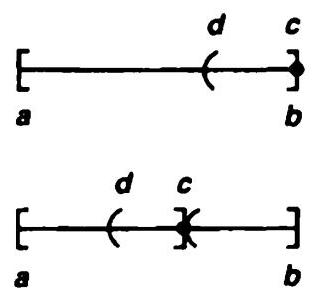
\includegraphics[width=0.2\textwidth]{images/24.1.jpg}
\end{center}
\hspace*{3em} 

Figure 24.1

\begin{center}
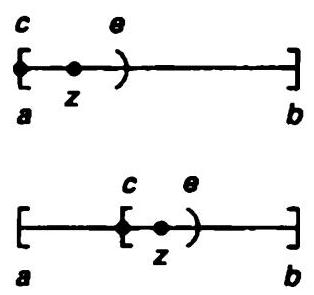
\includegraphics[width=0.2\textwidth]{images/24.2.jpg}
\end{center}
\hspace*{3em} 

Figure 24.2

Case 2. Suppose that \(c \in {A}_{0}\) . Then \(c \neq b\) , so either \(c = a\) or \(a < c < b\) . Because \({A}_{0}\) is open in \(\left\lbrack {a,b}\right\rbrack\) , there must be some interval of the form \(\lbrack c,e)\) contained in \({A}_{0}\) . See Figure 24.2. Because of order property (2) of the linear continuum \(L\) , we can choose a point \(z\) of \(L\) such that \(c < z < e\) . Then \(z \in {A}_{0}\) , contrary to the fact that \(c\) is an upper bound for \({A}_{0}\) .
\end{proof}

\begin{corollary} The real line \(\mathbb{R}\) is connected and so are intervals and rays in \(\mathbb{R}\) .
\end{corollary}

As an application, we prove the intermediate value theorem of calculus, suitably generalized.

\begin{theorem}[Intermediate value theorem] Let \(f: X \rightarrow Y\) be a continuous map, where \(X\) is a connected space and \(Y\) is an ordered set in the order topology. If a and \(b\) are two points of \(X\) and if \(r\) is a point of \(Y\) lying between \(f\left( a\right)\) and \(f\left( b\right)\) , then there exists a point \(c\) of \(X\) such that \(f\left( c\right) = r\) .

The intermediate value theorem of calculus is the special case of this theorem that occurs when we take \(X\) to be a closed interval in \(\mathbb{R}\) and \(Y\) to be \(\mathbb{R}\) .

\end{theorem}
\begin{proof}
Assume the hypotheses of the theorem. The sets

\[
A = f\left( X\right) \cap \left( {-\infty,r}\right) \;\text{ and }\;B = f\left( X\right) \cap \left( {r, + \infty }\right)
\]

are disjoint, and they are nonempty because one contains \(f\left( a\right)\) and the other contains \(f\left( b\right)\) . Each is open in \(f\left( X\right)\) , being the intersection of an open ray in \(Y\) with \(f\left( X\right)\) . If there were no point \(c\) of \(X\) such that \(f\left( c\right) = r\) , then \(f\left( X\right)\) would be the union of the sets \(A\) and \(B\) . Then \(A\) and \(B\) would constitute a separation of \(f\left( X\right)\) , contradicting the fact that the image of a connected space under a continuous map is connected.
\end{proof}

\begin{centeredblock}
\begin{example} One example of a linear continuum different from \(\mathbb{R}\) is the ordered square. We check the least upper bound property. (The second property of a linear continuum is trivial to check.) Let \(A\) be a subset of \(I \times I\) , let \({\pi }_{1}I \times I \rightarrow I\) be projection on the first coordinate; let \(b = \sup {\pi }_{1}\left( A\right)\) . If \(b \in {\pi }_{1}\left( A\right)\) , then \(A\) intersects the subset \(b \times I\) of \(I \times I\) . Because \(b \times I\) has the order type of \(I\) , the set \(A \cap \left( {b \times I}\right)\) will have a least upper bound \(b \times c\) , which will be the least upper bound of \(A\) . See Figure 24.3. If \(b \notin {\pi }_{1}\left( A\right)\) , then \(b \times 0\) is the least upper bound of \(A\) ; no element of the form \({b}^{\prime } \times c\) with \({b}^{\prime } < b\) can be an upper bound for \(A\) , for then \({b}^{\prime }\) would be an upper bound for \({\pi }_{l}\left( A\right)\) .

\begin{center}
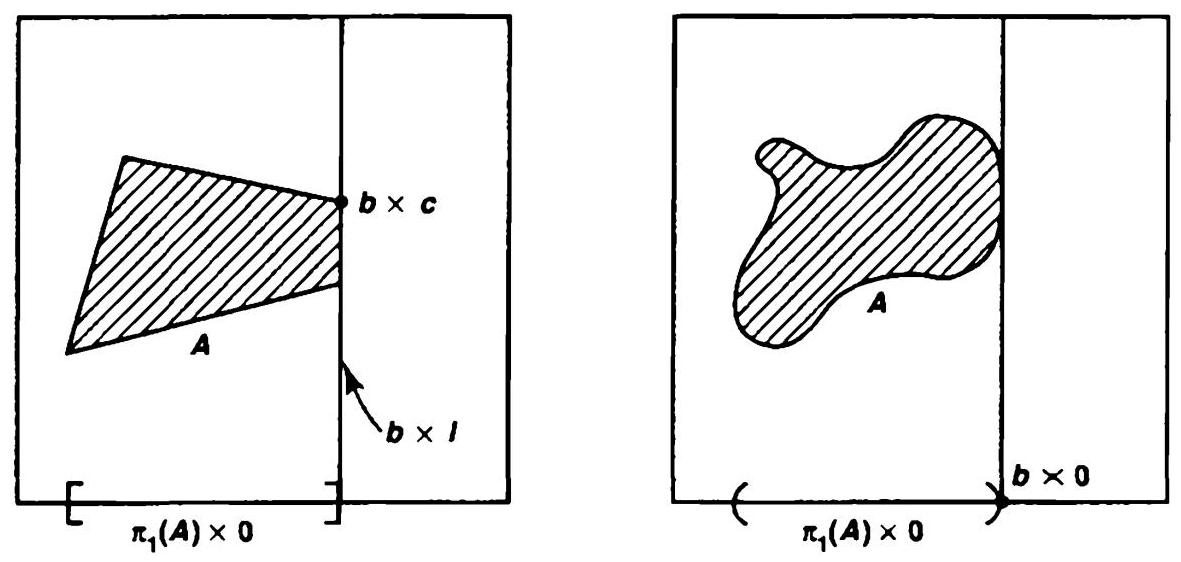
\includegraphics[width=1.0\textwidth]{images/24.3.jpg}
\end{center}
\hspace*{3em}

Figure 24.3
\end{example}
\end{centeredblock}

\begin{centeredblock}
\begin{example} If \(X\) is a well-ordered set, then \(X \times \lbrack 0,1)\) is a linear continuum in the dictionary order; this we leave to you to check. This set can be thought of as having been constructed by ``fitting in'' a set of the order type of(0,1)immediately following each element of \(X\) .
\end{example}
\end{centeredblock}

Connectedness of intervals in \(\mathbb{R}\) gives rise to an especially useful criterion for showing that a space \(X\) is connected; namely, the condition that every pair of points of \(X\) can be joined by a path in \(X\) :

\begin{definition} Given points \(x\) and \(y\) of the space \(X\) , a path in \(X\) from \(x\) to \(y\) is a continuous map \(f: \left\lbrack {a,b}\right\rbrack \rightarrow X\) of some closed interval in the real line into \(X\) , such that \(f\left( a\right) = x\) and \(f\left( b\right) = y\) . A space \(X\) is said to be path connected if every pair of points of \(X\) can be joined by a path in \(X\) .
\end{definition}


It is easy to see that a path-connected space \(X\) is connected. Suppose \(X = A \cup B\) is a separation of \(X\) . Let \(f: \left\lbrack {a,b}\right\rbrack \rightarrow X\) be any path in \(X\) . Being the continuous image of a connected set, the set \(f\left( \left\lbrack {a,b}\right\rbrack \right)\) is connected, so that it lies entirely in either \(A\) or \(B\) . Therefore, there is no path in \(X\) joining a point of \(A\) to a point of \(B\) , contrary to the assumption that \(X\) is path connected.

The converse does not hold; a connected space need not be path connected. See Examples 6 and 7 following.

\begin{centeredblock}
\begin{example} Define the unit ball \({B}^{n}\) in \({\mathbb{R}}^{n}\) by the equation

\[
{B}^{n} = \{ \mathbf{x} \mid \parallel \mathbf{x}\parallel \leq 1\}
\]

where

\[
\parallel \mathbf{x}\parallel = \begin{Vmatrix}\left( {{x}_{1},\ldots,{x}_{n}}\right) \end{Vmatrix} = {\left( {x}_{1}^{2} + \cdots + {x}_{n}^{2}\right) }^{1/2}
\]

The unit ball is path connected; given any two points \(\mathbf{x}\) and \(\mathbf{y}\) of \({B}^{n}\) , the straight-line path \(f: \left\lbrack {0,1}\right\rbrack \rightarrow {\mathbb{R}}^{n}\) defined by

\[
f\left( t\right) = \left( {1 - t}\right) x + {ty}
\]

lies in \({B}^{n}\) . For if \(x\) and \(y\) are in \({B}^{n}\) and \(t\) is in \(\left\lbrack {0,1}\right\rbrack\) ,

\[
\parallel f\left( t\right) \parallel \leq \left( {1 - t}\right) \parallel \mathbf{x}\parallel + t\parallel \mathbf{y}\parallel \leq 1.
\]

A similar argument shows that every open ball \({B}_{d}\left( {\mathbf{x},\epsilon }\right)\) and every closed ball \({\bar{B}}_{d}\left( {\mathbf{x},\epsilon }\right)\) in \({\mathbb{R}}^{n}\) is path connected.
\end{example}
\end{centeredblock}

\begin{centeredblock}
\begin{example} Define punctured euclidean space to be the space \({\mathbb{R}}^{n} - \{ \mathbf{0}\}\) , where0is the origin in \({\mathbb{R}}^{n}\) . If \(n > 1\) , this space is path connected. Given \(\mathbf{x}\) and \(\mathbf{y}\) different from 0, we can join \(x\) and \(y\) by the straight-line path between them if that path does not go through the origin. Otherwise, we can choose a point \(\mathbf{z}\) not on the line joining \(\mathbf{x}\) and \(\mathbf{y}\) , and take the broken-line path from \(x\) to \(z\) , and then from \(z\) to \(y\)
\end{example}
\end{centeredblock}

\begin{centeredblock}
\begin{example} Define the unit sphere \({S}^{n - 1}\) in \({\mathbb{R}}^{n}\) by the equation

\[
{S}^{n - 1} = \{ \mathbf{x} \mid \parallel \mathbf{x}\parallel = 1\} .
\]

If \(n > 1\) , it is path connected. For the map \(g: {\mathbb{R}}^{n} - \{ \mathbf{0}\} \rightarrow {S}^{n - 1}\) defined by \(g\left( \mathbf{x}\right) = \mathbf{x}/\parallel \mathbf{x}\parallel\) is continuous and surjective; and it is easy to show that the continuous image of a path-connected space is path connected.
\end{example}
\end{centeredblock}

\begin{centeredblock}
\begin{example} The ordered square \({I}_{o}^{2}\) is connected but not path connected.

Being a linear continuum, the ordered square is connected. Let \(p = 0 \times 0\) and \(q =\) \(1 \times 1\) . We suppose there is a path \(f: \left\lbrack {a,b}\right\rbrack \rightarrow {I}_{o}^{2}\) joining \(p\) and \(q\) and derive a contradiction. The image set \(f\left( \left\lbrack {a,b}\right\rbrack \right)\) must contain every point \(x \times y\) of \({I}_{o}^{2}\) , by the intermediate value theorem. Therefore, for each \(x \in I\) , the set

\[
{U}_{x} = {f}^{-1}\left( {x \times \left( {0,1}\right) }\right)
\]

is a nonempty subset of \(\left\lbrack {a,b}\right\rbrack\) ; by continuity, it is open in \(\left\lbrack {a,b}\right\rbrack\) . See Figure 24.4. Choose, for each \(x \in I\) , a rational number \({q}_{x}\) beloriging to \({U}_{x}\) . Since the sets \({U}_{x}\) are disjoint, the map \(x \rightarrow {q}_{x}\) is an injective mapping of \(I\) into \(\mathbb{Q}\) . This contradicts the fact that the interval \(I\) is uncountable (which we shall prove later)
\end{example}
\end{centeredblock}

\begin{centeredblock}
\begin{example} Let \(S\) denote the following subset of the plane.

\[
S = \{ x \times \sin \left( {1/x}\right) \mid 0 < x \leq 1\} .
\]

Because \(S\) is the image of the connected set \((0,1\rbrack\) under a continuous map, \(S\) is connected. Therefore, its closure \(\bar{S}\) in \({\mathbb{R}}^{2}\) is also connected. The set \(\bar{S}\) is a classical example in topology called the topologist’s sine curve. It is illustrated in Figure 24.5; it equals the union of \(S\) and the vertical interval \(0 \times \left\lbrack {-1,1}\right\rbrack\) . We show that \(\bar{S}\) is not path connected.

\begin{center}
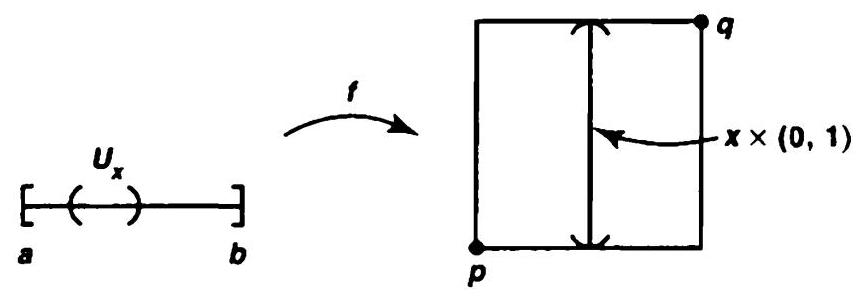
\includegraphics[width=0.7\textwidth]{images/24.4.jpg}
\end{center}
\hspace*{3em} 

Figure 24.4

Suppose there is a path \(f.\left\lbrack {a,c}\right\rbrack \rightarrow \bar{S}\) beginning at the origin and ending at a point of \(S\) . The set of those \(t\) for which \(f\left( t\right) \in 0 \times \left\lbrack {-1,1}\right\rbrack\) is closed, so it has a largest element \(b\) . Then \(f: \left\lbrack {b,c}\right\rbrack \rightarrow \bar{S}\) is a path that maps \(b\) into the vertical interval \(0 \times \left\lbrack {-1,1}\right\rbrack\) and maps the other points of \(\left\lbrack {b,c}\right\rbrack\) to points of \(S\) .

Replace \(\left\lbrack {b,c}\right\rbrack\) by \(\left\lbrack {0,1}\right\rbrack\) for convenience; let \(f\left( t\right) = \left( {x\left( t\right) ,y\left( t\right) }\right)\) . Then \(x\left( 0\right) = 0\) , while \(x\left( t\right) > 0\) and \(y\left( t\right) = \sin \left( {1/x\left( t\right) }\right)\) for \(t > 0\) . We show there is a sequence of points \({t}_{n} \rightarrow 0\) such that \(y\left( {t}_{n}\right) = {\left( -1\right) }^{n}\) . Then the sequence \(y\left( {t}_{n}\right)\) does not converge, contradicting continuity of \(f\) .

To find \({t}_{n}\) , we proceed as follows: Given \(n\) , choose \(u\) with \(0 < u < x\left( {1/n}\right)\) such that \(\sin \left( {1/u}\right) = {\left( -1\right) }^{n}\) . Then use the intermediate value theorem to find \({t}_{n}\) with \(0 < {t}_{n} < 1/n\) such that \(x\left( {t}_{n}\right) = u\) .

\begin{center}
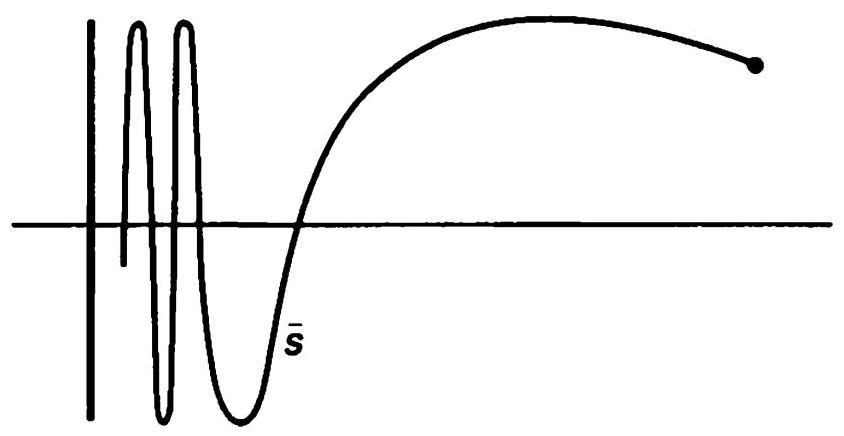
\includegraphics[width=0.7\textwidth]{images/24.5.jpg}
\end{center}
\hspace*{3em} 

Figure 24.5
\end{example}
\end{centeredblock}

\section*{Exercises}

1. (a) Show that no two of the spaces \(\left( {0,1}\right) ,(0,1\rbrack\) , and \(\left\lbrack {0,1}\right\rbrack\) are homeomorphic. [Hint: What happens if you remove a point from each of these spaces?)]

(b) Suppose that there exist imbeddings \(f: X \rightarrow Y\) and \(g: Y \rightarrow X\) . Show by means of an example that \(X\) and \(Y\) need not be homeomorphic.

(c) Show \({\mathbb{R}}^{n}\) and \(\mathbb{R}\) are not homeomorphic if \(n > 1\) .

2. Let \(f: {S}^{1} \rightarrow \mathbb{R}\) be a continuous map. Show there exists a point \(x\) of \({S}^{1}\) such that \(f\left( x\right) = f\left( {-x}\right)\) .

3. Let \(f: X \rightarrow X\) be continuous. Show that if \(X = \left\lbrack {0,1}\right\rbrack\) , there is a point \(x\) such that \(f\left( x\right) = x\) . The point \(x\) is called a fixed point of \(f\) . What happens if \(X\) equals \(\lbrack 0,1)\) or \(\left( {0,1}\right) {}^{7}\)

4. Let \(X\) be an ordered set in the order topology. Show that if \(X\) is connected, then \(X\) is a linear continuum.

5. Consider the following sets in the dictionary order. Which are linear continua?

(a) \({\mathbb{Z}}_{ + } \times \lbrack 0,1)\)

(b) \(\lbrack 0,1) \times {\mathbb{Z}}_{ + }\)

(c) \(\lbrack 0,1) \times \left\lbrack {0,1}\right\rbrack\)

(d) \(\left\lbrack {0,1}\right\rbrack \times \lbrack 0,1)\)

6. Show that if \(X\) is a well-ordered set, then \(X \times \lbrack 0,1)\) in the dictionary order is a linear continuum.

7. (a) Let \(X\) and \(Y\) be ordered sets in the order topology. Show that if \(f: X \rightarrow Y\) is order preserving and surjective, then \(f\) is a homeomorphism.

(b) Let \(X = Y = {\overline{\mathbb{R}}}_{ + }\) . Given a positive integer \(n\) , show that the function \(f\left( x\right) =\) \({x}^{n}\) is order preserving and surjective. Conclude that its inverse, the nth root function, is continuous.

(c) Let \(X\) be the subspace \(\left( {-\infty, - 1}\right) \cup \lbrack 0,\infty )\) of \(\mathbb{R}\) . Show that the function \(f: X \rightarrow \mathbb{R}\) defined by setting \(f\left( x\right) = x + 1\) if \(x < - 1\) , and \(f\left( x\right) = x\) if \(x \geq 0\) , is order preserving and surjective. Is \(f\) a homeomorphism? Compare with (a).

8. (a) Is a product of path-connected spaces necessarily path connected?

(b) If \(A \subset X\) and \(A\) is path connected, is \(\bar{A}\) necessarily path connected?

(c) If \(f: X \rightarrow Y\) is continuous and \(X\) is path connected, is \(f\left( X\right)\) necessarily path connected?

(d) If \(\left\{ {A}_{\alpha }\right\}\) is a collection of path-connected subspaces of \(X\) and if \(\bigcap {A}_{\alpha } \neq \varnothing\) , is \(\bigcup {A}_{\alpha }\) necessarily path connected?

9. Assume that \(\mathbb{R}\) is uncountable. Show that if \(A\) is a countable subset of \({\mathbb{R}}^{2}\) , then \({\mathbb{R}}^{2} - A\) is path connected. [Hint: How many lines are there passing through a given point of \({\mathbb{R}}^{2}\) ?]

10. Show that if \(U\) is an open connected subspace of \({\mathbb{R}}^{2}\) , then \(U\) is path connected. [Hint: Show that given \({x}_{0} \in U\) , the set of points that can be joined to \({x}_{0}\) by a path in \(U\) is both open and closed in \(U\) .]

11. If \(A\) is a connected subspace of \(X\) , does it follow that Int \(A\) and Bd \(A\) are connected? Does the converse hold? Justify your answers.

*12. Recall that \({S}_{\Omega }\) denotes the minimal uncountable well-ordered set. Let \(L\) denote the ordered set \({S}_{\Omega } \times \lbrack 0,1)\) in the dictionary order, with its smallest element deleted. The set \(L\) is a classical example in topology called the long line.

\begin{theorem} The long line is path connected and locally homeomorphic to \(\mathbb{R}\) , but it cannot be imbedded in \(\mathbb{R}\) .

(a) Let \(X\) be an ordered set; let \(a < b < c\) be points of \(X\) . Show that \(\lbrack a,c)\) has the order type of \(\lbrack 0,1)\) if and only if both \(\lbrack a,b)\) and \(\lbrack b,c)\) have the order type of \(\lbrack 0,1)\)

(b) Let \(X\) be an ordered set. Let \({x}_{0} < {x}_{1} < \cdots\) be an increasing sequence of points of \(X\) ; suppose \(b = \sup \left\{ {x}_{t}\right\}\) Show that \(\left\lbrack {{x}_{0},b}\right)\) has the order type of \(\lbrack 0,1)\) if and only if each interval \(\left\lbrack {{x}_{i},{x}_{i + 1}}\right)\) has the order type of \(\lbrack 0,1)\) .

(c) Let \({a}_{0}\) denote the smallest element of \({S}_{\Omega }\) . For each element \(a\) of \({S}_{\Omega }\) different from \({a}_{0}\) , show that the interval \(\left\lbrack {{a}_{0} \times 0,a \times 0}\right)\) of \({S}_{\Omega } \times \lbrack 0,1)\) has the order type of \(\lbrack 0,1)\) . [Hint: Proceed by transfinite induction. Either \(a\) has an immediate predecessor in \({S}_{\Omega }\) , or there is an increasing sequence \({a}_{t}\) in \({S}_{\Omega }\) with \(a = \sup \left\{ {a}_{i}\right\}\) .

(d) Show that \(L\) is path connected.

(e) Show that every point of \(L\) has a neighborhood homeomorphic with an open interval in \(\mathbb{R}\) .

(f) Show that \(L\) cannot be imbedded in \(\mathbb{R}\) , or indeed in \({\mathbb{R}}^{n}\) for any \(n\) . [Hint: Any subspace of \({\mathbb{R}}^{n}\) has a countable basis for its topology.]

\end{theorem}
\section*{*§ 25 Components and Local Connectedness \protect\sectionDagger}

Given an arbitrary space \(X\) , there is a natural way to break it up into pieces that are connected (or path connected). We consider that process now.

\begin{definition} Given \(X\) , define an equivalence relation on \(X\) by setting \(x \sim y\) if there is a connected subspace of \(X\) containing both \(x\) and \(y\) . The equivalence classes are called the components (or the ``connected components'') of \(X\) .
\end{definition}


Symmetry and reflexivity of the relation are obvious. Transitivity follows by noting that if \(A\) is a connected subspace containing \(x\) and \(y\) , and if \(B\) is a connected subspace containing \(y\) and \(z\) , then \(A \cup B\) is a subspace containing \(x\) and \(z\) that is connected because \(A\) and \(B\) have the point \(y\) in common.

The components of \(X\) can also be described as follows:

\begin{theorem} The components of \(X\) are connected disjoint subspaces of \(X\) whose union is \(X\) , such that each nonempty connected subspace of \(X\) intersects only one of them.

\end{theorem}
\begin{proof}
Being equivalence classes, the components of \(X\) are disjoint and their union is \(X\) . Each connected subspace \(A\) of \(X\) intersects only one of them. For if \(A\) intersects the components \({C}_{1}\) and \({C}_{2}\) of \(X\) , say in points \({x}_{1}\) and \({x}_{2}\) , respectively, then \({x}_{1} \sim {x}_{2}\) by definition; this cannot happen unless \({C}_{1} = {C}_{2}\) .

\customfootnote
{
${}^{\dagger}$ This section will be assumed in Part II of the book.
}

To show the component \(C\) is connected, choose a point \({x}_{0}\) of \(C\) . For each point \(x\) of \(C\) , we know that \({x}_{0} \sim x\) , so there is a connected subspace \({A}_{x}\) containing \({x}_{0}\) and \(x\) . By the result just proved, \({A}_{x} \subset C\) . Therefore,

\[
C = \mathop{\bigcup }\limits_{{x \in C}}{A}_{x}
\]

Since the subspaces \({A}_{x}\) are connected and have the point \({x}_{0}\) in common, their union is connected.
\end{proof}

\begin{definition} We define another equivalence relation on the space \(X\) by defining \(x \sim y\) if there is a path in \(X\) from \(x\) to \(y\) . The equivalence classes are called the path components of \(X\) .
\end{definition}


Let us show this is an equivalence relation. First we note that if there exists a path \(f: \left\lbrack {a,b}\right\rbrack \rightarrow X\) from \(x\) to \(y\) whose domain is the interval \(\left\lbrack {a,b}\right\rbrack\) , then there is also a path \(g\) from \(x\) to \(y\) having the closed interval \(\left\lbrack {c,d}\right\rbrack\) as its domain. (This follows from the fact that any two closed intervals in \(\mathbb{R}\) are homeomorphic.) Now the fact that \(x \sim x\) for each \(x\) in \(X\) follows from the existence of the constant path \(f: \left\lbrack {a,b}\right\rbrack \rightarrow X\) defined by the equation \(f\left( t\right) = x\) for all \(t\) . Symmetry follows from the fact that if \(f: \left\lbrack {0,1}\right\rbrack \rightarrow X\) is a path from \(x\) to \(y\) , then the ``reverse path'' \(g: \left\lbrack {0,1}\right\rbrack \rightarrow X\) defined by \(g\left( t\right) = f\left( {1 - t}\right)\) is a path from \(y\) to \(x\) . Finally, transitivity is proved as follows: Let \(f: \left\lbrack {0,1}\right\rbrack \rightarrow X\) be a path from \(x\) to \(y\) , and let \(g.\left\lbrack {1,2}\right\rbrack \rightarrow X\) be a path from \(y\) to \(z\) . We can ``paste \(f\) and \(g\) together'' to get a path \(h: \left\lbrack {0,2}\right\rbrack \rightarrow X\) from \(x\) to \(z\) ; the path \(h\) will be continuous by the ``pasting lemma,'' Theorem 18.3.

One has the following theorem, whose proof is similar to that of the theorem preceding:

\begin{theorem} The path components of \(X\) are path-connected disjoint subspaces of \(X\) whose union is \(X\) , such that each nonempty path-connected subspace of \(X\) intersects only one of them.

Note that each component of a space \(X\) is closed in \(X\) , since the closure of a connected subspace of \(X\) is connected. If \(X\) has only finitely many components, then each component is also open in \(X\) , since its complement is a finite union of closed sets But in general the components of \(X\) need not be open in \(X\) .

One can say even less about the path components of \(X\) , for they need be neither open nor closed in \(X\) . Consider the following examples:

\begin{centeredblock}
\begin{example} If \(\mathbb{Q}\) is the subspace of \(\mathbb{R}\) consisting of the rational numbers, then each component of \(\mathbb{Q}\) consists of a single point. None of the components of \(\mathbb{Q}\) are open in \(\mathbb{Q}\) .
\end{example}
\end{centeredblock}

\begin{centeredblock}
\begin{example} The ``topologist's sine curve'' \(\bar{S}\) of the preceding section is a space that has a single component (since it is connected) and two path components One path component is the curve \(S\) and the other is the vertical interval \(V = 0 \times \left\lbrack {-1,1}\right\rbrack\) . Note that \(S\) is open in \(\bar{S}\) but not closed, while \(V\) is closed but not open

If one forms a space from \(\widetilde{S}\) by deleting all points of \(V\) having rational second coordinate, one obtains a space that has only one component but uncountably many path components.
\end{example}
\end{centeredblock}

Connectedness is a useful property for a space to possess. But for some purposes, it is more important that the space satisfy a connectedness condition locally. Roughly speaking, local connectedness means that each point has ``arbitrarily small'' neighborhoods that are connected. More precisely, one has the following definition:

\begin{definition} A space \(X\) is said to be locally connected at \(x\) if for every neighborhood \(U\) of \(x\) , there is a connected neighborhood \(V\) of \(x\) contained in \(U\) If \(X\) is locally connected at each of its points, it is said simply to be locally connected. Similarly, a space \(X\) is said to be locally path connected at \(x\) if for every neighborhood \(U\) of \(x\) , there is a path-connected neighborhood \(V\) of \(x\) contained in \(U\) . If \(X\) is locally path connected at each of its points, then it is said to be locally path connected.
\end{definition}


\begin{centeredblock}
\begin{example} Each interval and each ray in the real line is both connected and locally connected The subspace \(\left\lbrack {-1,0)\cup (0,1}\right\rbrack\) of \(\mathbb{R}\) is not connected, but it is locally connected The topologist’s sine curve is connected but not locally connected. The rationals \(\mathbb{Q}\) are neither connected nor locally connected.
\end{example}
\end{centeredblock}

\end{theorem}
\begin{theorem} A space \(X\) is locally connected if and only if for every open set \(U\) of \(X\) , each component of \(U\) is open in \(X\) .

\end{theorem}
\begin{proof}
Suppose that \(X\) is locally connected; let \(U\) be an open set in \(X\) ; let \(C\) be a component of \(U\) If \(x\) is a point of \(C\) , we can choose a connected neighborhood \(V\) of \(x\) such that \(V \subset U\) . Since \(V\) is connected, it must lie entirely in the component \(C\) of \(U\) . Therefore, \(C\) is open in \(X\) .

Conversely, suppose that components of open sets in \(X\) are open. Given a point \(x\) of \(X\) and a neighborhood \(U\) of \(x\) , let \(C\) be the component of \(U\) containing \(x\) . Now \(C\) is connected; since it is open in \(X\) by hypothesis, \(X\) is locally connected at \(x\) .

A similar proof holds for the following theorem:

\begin{theorem} A space \(X\) is locally path connected if and only if for every open set \(U\) of \(X\) , each path component of \(U\) is open in \(X\) .

The relation between path components and components is given in the following theorem:

\end{theorem}
\begin{theorem} If \(X\) is a topological space, each path component of \(X\) lies in a component of \(X\) If \(X\) is locally path connected, then the components and the path components of \(X\) are the same.

\({Proof}\) . Let \(C\) be a component of \(X\) ; let \(x\) be a point of \(C\) ; let \(P\) be the path component of \(X\) containing \(x\) . Since \(P\) is connected, \(P \subset C\) . We wish to show that if \(X\) is locally path connected, \(P = C\) . Suppose that \(P \subsetneq C\) . Let \(Q\) denote the union of all the path components of \(X\) that are different from \(P\) and intersect \(C\) , each of them necessarily lies in \(C\) , so that

\[
C = P \cup Q\text{ . }
\]

Because \(X\) is locally path connected, each path component of \(X\) is open in \(X\) . Therefore, \(P\) (which is a path component) and \(Q\) (which is a union of path components) are open in \(X\) , so they constitute a separation of \(C\) . This contradicts the fact that \(C\) is connected.

\end{theorem}
\end{proof}
\section*{Exercises}

1. What are the components and path components of \({\mathbb{R}}_{\ell }\) ? What are the continuous maps \(f: \mathbb{R} \rightarrow {\mathbb{R}}_{\ell }\) ?

2. (a) What are the components and path components of \({\mathbb{R}}^{\omega }\) (in the product topology)?

(b) Consider \({\mathbb{R}}^{\omega }\) in the uniform topology. Show that \(\mathbf{x}\) and \(\mathbf{y}\) lie in the same component of \({\mathbb{R}}^{\omega }\) if and only if the sequence

\[
\mathbf{x} - \mathbf{y} = \left( {{x}_{1} - {y}_{1},{x}_{2} - {y}_{2},\ldots }\right)
\]

is bounded. [Hint: It suffices to consider the case where \(\mathbf{y} = \mathbf{0}\) .]

(c) Give \({\mathbb{R}}^{\omega }\) the box topology. Show that \(\mathbf{x}\) and \(\mathbf{y}\) lie in the same component of \({\mathbb{R}}^{\omega }\) if and only if the sequence \(\mathbf{x} - \mathbf{y}\) is ``eventually zero.'' [Hint: If \(\mathbf{x} - \mathbf{y}\) is not eventually zero, show there is homeomorphism \(h\) of \({\mathbb{R}}^{\omega }\) with itself such that \(h\left( \mathbf{x}\right)\) is bounded and \(h\left( \mathbf{y}\right)\) is unbounded.]

3. Show that the ordered square is locally connected but not locally path connected. What are the path components of this space?

4. Let \(X\) be locally path connected. Show that every connected open set in \(X\) is path connected.

5. Let \(X\) denote the rational points of the interval \(\left\lbrack {0,1}\right\rbrack \times 0\) of \({\mathbb{R}}^{2}\) . Let \(T\) denote the union of all line segments joining the point \(p = 0 \times 1\) to points of \(X\) .

(a) Show that \(T\) is path connected, but is locally connected only at the point \(p\) .

(b) Find a subset of \({\mathbb{R}}^{2}\) that is path connected but is locally connected at none of its points.

6. A space \(X\) is said to be weakly locally connected at \(x\) if for every neighborhood \(U\) of \(x\) , there is a connected subspace of \(X\) contained in \(U\) that contains a neighborhood of \(x\) . Show that if \(X\) is weakly locally connected at each of its points, then \(X\) is locally connected. [Hint: Show that components of open sets are open.]

7. Consider the ``infinite broom'' \(X\) pictured in Figure 25.1. Show that \(X\) is not locally connected at \(p\) , but is weakly locally connected at \(p\) . [Hint: Any connected neighborhood of \(p\) must contain all the points \({a}_{i}\) .]

\begin{center}
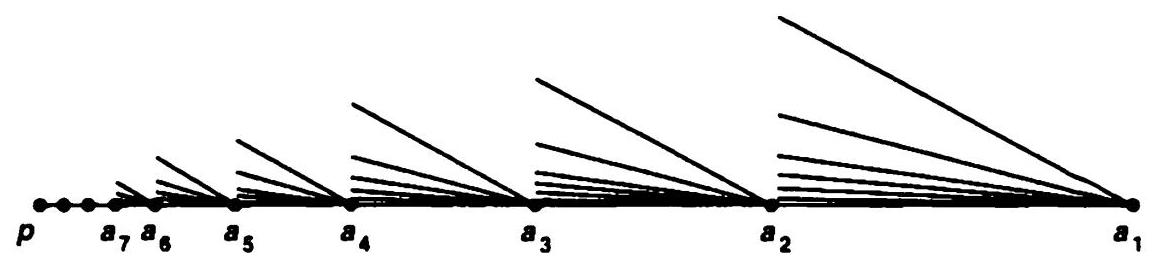
\includegraphics[width=1.0\textwidth]{images/25.1.jpg}
\end{center}
\hspace*{3em} 

Figure 25.1

8. Let \(p: X \rightarrow Y\) be a quotient map. Show that if \(X\) is locally connected, then \(Y\) is locally connected. [Hint: If \(C\) is a component of the open set \(U\) of \(Y\) , show that \({p}^{-1}\left( C\right)\) is a union of components of \({p}^{-1}\left( U\right)\) .]

9. Let \(G\) be a topological group; let \(C\) be the component of \(G\) containing the identity element \(e\) . Show that \(C\) is a normal subgroup of \(G\) . [Hint: If \(x \in G\) , then \({xC}\) is the component of \(G\) containing \(x\) .]

10. Let \(X\) be a space. Let us define \(x \sim y\) if there is no separation \(X = A \cup B\) of \(X\) into disjoint open sets such that \(x \in A\) and \(y \in B\) .

(a) Show this relation is an equivalence relation. The equivalence classes are called the quasicomponents of \(X\) .

(b) Show that each component of \(X\) lies in a quasicomponent of \(X\) , and that the components and quasicomponents of \(X\) are the same if \(X\) is locally connected.

(c) Let \(K\) denote the set \(\left\{ {1/n \mid n \in {\mathbb{Z}}_{ + }}\right\}\) and let \(- K\) denote the set \(\{ - 1/n \mid n \in\) \(\left. {\mathbb{Z}}_{ + }\right\}\) . Determine the components, path components, and quasicomponents of the following subspaces of \({\mathbb{R}}^{2}\) :

\[
A = \left( {K \times \left\lbrack {0,1}\right\rbrack }\right) \cup \{ 0 \times 0\} \cup \{ 0 \times 1\} .
\]

\[
B = A \cup \left( {\left\lbrack {0,1}\right\rbrack \times \{ 0\rbrack }\right) \text{ . }
\]

\[
C = \left( {K \times \left\lbrack {0,1}\right\rbrack }\right) \cup \left( {-K \times \left\lbrack {-1,0}\right\rbrack }\right) \cup \left( {\left\lbrack {0,1}\right\rbrack \times - K}\right) \cup \left( {\left\lbrack {-1,0}\right\rbrack \times K}\right) .
\]

\section*{§ 26 Compact Spaces}

The notion of compactness is not nearly so natural as that of connectedness. From the beginnings of topology, it was clear that the closed interval \(\left\lbrack {a,b}\right\rbrack\) of the real line had a certain property that was crucial for proving such theorems as the maximum value theorem and the uniform continuity theorem. But for a long time, it was not clear how this property should be formulated for an arbitrary topological space It used to be thought that the crucial property of \(\left\lbrack {a,b}\right\rbrack\) was the fact that every infinite subset of \(\left\lbrack {a,b}\right\rbrack\) has a limit point, and this property was the one dignified with the name of compactness. Later, mathematicians realized that this formulation does not lie at the heart of the matter, but rather that a stronger formulation, in terms of open coverings of the space, is more central. The latter formulation is what we now call compactness. It is not as natural or intuitive as the former; some familiarity with it is needed before its usefulness becomes apparent.

\begin{definition} A collection \(\mathcal{A}\) of subsets of a space \(X\) is said to cover \(X\) , or to be a covering of \(X\) , if the union of the elements of \(\mathcal{A}\) is equal to \(X\) . It is called an open covering of \(X\) if its elements are open subsets of \(X\) .
\end{definition}


\begin{definition} A space \(X\) is said to be compact if every open covering \(\mathcal{A}\) of \(X\) contains a finite subcollection that also covers \(X\) .
\end{definition}


\begin{centeredblock}
\begin{example} The real line \(\mathbb{R}\) is not compact, for the covering of \(\mathbb{R}\) by open intervals

\[
\mathcal{A} = \{ \left( {n,n + 2}\right) \mid n \in \mathbb{Z}\}
\]

contains no finite subcollection that covers \(\mathbb{R}\) .
\end{example}
\end{centeredblock}

\begin{centeredblock}
\begin{example} The following subspace of \(\mathbb{R}\) is compact:

\[
X = \{ 0\} \cup \{ 1/n \mid n \in {\mathbb{Z}}_{ + }\} .
\]

Given an open covering \(\mathcal{A}\) of \(X\) , there is an element \(U\) of \(\mathcal{A}\) containing 0. The set \(U\) contains all but finitely many of the points \(1/n\) ; choose, for each point of \(X\) not in \(U\) , an element of \(\mathcal{A}\) containing it. The collection consisting of these elements of \(\mathcal{A}\) , along with the element \(U\) , is a finite subcollection of \(\mathcal{A}\) that covers \(X\) .
\end{example}
\end{centeredblock}

\begin{centeredblock}
\begin{example} Any space \(X\) containing only finitely many points is necessarily compact, because in this case every open covering of \(X\) is finite.
\end{example}
\end{centeredblock}

\begin{centeredblock}
\begin{example} The interval \((0,1\rbrack\) is not compact; the open covering

\[
\mathcal{A} = \left\{ {(l/n,1\rbrack \mid n \in {\mathbb{Z}}_{ + }}\right\}
\]

contains no finite subcollection covering \((0,1\}\) . Nor is the interval(0,1)compact; the same argument applies. On the other hand, the interval \(\left\lbrack {0,1}\right\rbrack\) is compact; you are probably already famuliar with this fact from analysis. In any case, we shall prove it shortly.
\end{example}
\end{centeredblock}

In general, it takes some effort to decide whether a given space is compact or not. First we shall prove some general theorems that show us how to construct new compact spaces out of existing ones. Then in the next section we shall show certain specific spaces are compact. These spaces include all closed intervals in the real line, and all closed and bounded subsets of \({\mathbb{R}}^{n}\) .

Let us first prove some facts about subspaces. If \(Y\) is a subspace of \(X\) , a collection \(\mathcal{A}\) of subsets of \(X\) is said to cover \(Y\) if the union of its elements contains \(Y\) .

\begin{lemma} Let \(Y\) be a subspace of \(X\) . Then \(Y\) is compact if and only if every covering of \(Y\) by sets open in \(X\) contains a finite subcollection covering \(Y\) .
\end{lemma}

\begin{proof}
Suppose that \(Y\) is compact and \(\mathcal{A} = {\left\{ {A}_{\alpha }\right\} }_{\alpha \in J}\) is a covering of \(Y\) by sets open in \(X\) . Then the collection

\[
\left\{ {{A}_{\alpha } \cap Y \mid \alpha \in J}\right\}
\]

is a covering of \(Y\) by sets open in \(Y\) ; hence a finite subcollection

\[
\left\{ {{A}_{{\alpha }_{1}} \cap Y,\ldots,{A}_{{\alpha }_{n}} \cap Y}\right\}
\]

covers \(Y\) . Then \(\left\{ {{A}_{{\alpha }_{1}},\ldots,{A}_{{\alpha }_{n}}}\right\}\) is a subcollection of \(\mathcal{A}\) that covers \(Y\) .

Conversely, suppose the given condition holds; we wish to prove \(Y\) compact. Let \({\mathcal{A}}^{\prime } = \left\{ {A}_{\alpha }^{\prime }\right\}\) be a covering of \(Y\) by sets open in \(Y\) . For each \(\alpha\) , choose a set \({A}_{\alpha }\) open in \(X\) such that

\[
{A}_{\alpha }^{\prime } = {A}_{\alpha } \cap Y
\]

The collection \(\mathcal{A} = \left\{ {A}_{\alpha }\right\}\) is a covering of \(Y\) by sets open in \(X\) By hypothesis, some finite subcollection \(\left\{ {{A}_{{\alpha }_{1}},\ldots,{A}_{{\alpha }_{n}}}\right\}\) covers \(Y\) . Then \(\left\{ {{A}_{{\alpha }_{1}}^{\prime },\ldots,{A}_{{\alpha }_{n}}^{\prime }}\right\}\) is a subcollection of \({\mathcal{A}}^{\prime }\) that covers \(Y\)
\end{proof}

\section*{Theorem 26.2. Every closed subspace of a compact space is compact.}

\begin{proof}
Let \(Y\) be a closed subspace of the compact space \(X\) . Given a covering \(\mathcal{A}\) of \(Y\) by sets open in \(X\) , let us form an open covering \(\mathcal{B}\) of \(X\) by adjoining to \(\mathcal{A}\) the single open set \(X - Y\) , that is,

\[
\mathcal{B} = \mathcal{A} \cup \{ X - Y\} .
\]

Some finite subcollection of \(\mathcal{B}\) covers \(X\) . If this subcollection contains the set \(X - Y\) , discard \(X - Y\) ; otherwise, leave the subcollection alone. The resulting collection is a finite subcollection of \(\mathcal{A}\) that covers \(Y\) .
\end{proof}

\section*{Theorem 26.3. Every compact subspace of a Hausdorff space is closed.}

\begin{proof}
Let \(Y\) be a compact subspace of the Hausdorff space \(X\) . We shall prove that \(X - Y\) is open, so that \(Y\) is closed.

Let \({x}_{0}\) be a point of \(X - Y\) . We show there is a neighborhood of \({x}_{0}\) that is disjoint from \(Y\) . For each point \(y\) of \(Y\) , let us choose disjoint neighborhoods \({U}_{y}\) and \({V}_{y}\) of the points \({x}_{0}\) and \(y\) , respectively (using the Hausdorff condition). The collection \(\left\{ {{V}_{y} \mid y \in }\right.\) \(Y\}\) is a covering of \(Y\) by sets open in \(X\) ; therefore, finitely many of them \({V}_{{y}_{1}},\ldots,{V}_{{y}_{n}}\) cover \(Y\) . The open set

\[
V = {V}_{{y}_{1}} \cup \cdot \cup {V}_{{y}_{n}}
\]

contains \(Y\) , and it is disjoint from the open set

\[
U = {U}_{{y}_{1}} \cap \cdots \cap {U}_{{y}_{n}}
\]

formed by taking the intersection of the corresponding neighborhoods of \({x}_{0}\) . For if \(z\) is a point of \(V\) , then \(z \in {V}_{{y}_{i}}\) for some \(i\) , hence \(z \notin {U}_{{y}_{i}}\) and so \(z \notin U\) . See Figure 26.1.

Then \(U\) is a neighborhood of \({x}_{0}\) disjoint from \(Y\) , as desired.

\begin{center}
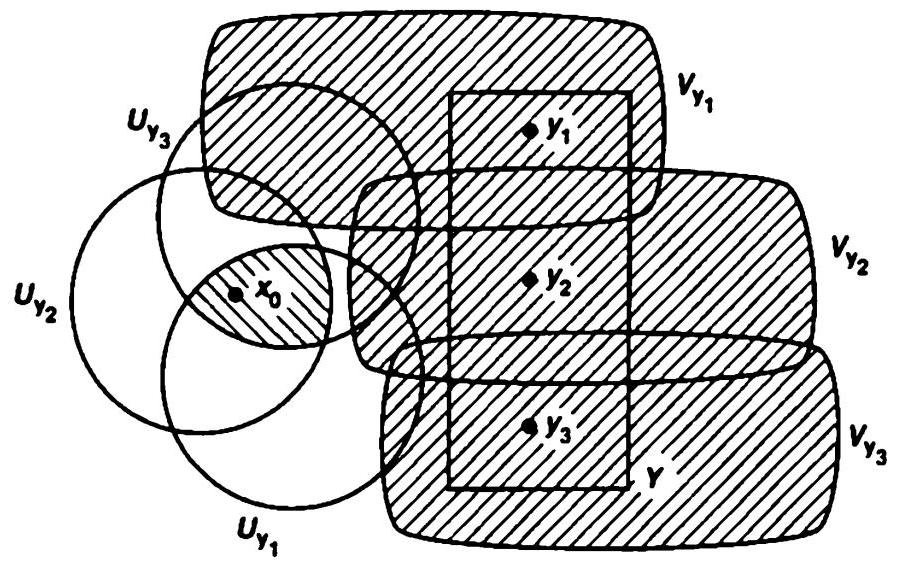
\includegraphics[width=0.8\textwidth]{images/26.1.jpg}
\end{center}
\hspace*{3em} 

Figure 26.1

The statement we proved in the course of the preceding proof will be useful to us later, so we repeat it here for reference purposes:
\end{proof}

\begin{lemma} If \(Y\) is a compact subspace of the Hausdorff space \(X\) and \({x}_{0}\) is not in \(Y\) , then there exist disjoint open sets \(U\) and \(V\) of \(X\) containing \({x}_{0}\) and \(Y\) , respectively.
\end{lemma}

\begin{centeredblock}
\begin{example} Once we prove that the interval \(\left\lbrack {a,b}\right\rbrack\) in \(\mathbb{R}\) is compact, it follows from Theorem 26 2 that any closed subspace of \(\left\lbrack {a,b}\right\rbrack\) is compact. On the other hand, it follows from Theorem 26.3 that the intervals \((a,b\rbrack\) and(a, b)in \(\mathbb{R}\) cannot be compact (which we knew already) because they are not closed in the Hausdorff space \(\mathbf{R}\)
\end{example}
\end{centeredblock}

\begin{centeredblock}
\begin{example} One needs the Hausdorff condition in the hypothesis of Theorem 263 Consider, for example, the finite complement topology on the real line The only proper subsets of \(\mathbb{R}\) that are closed in this topology are the finite sets. But every subset of \(\mathbb{R}\) is compact in this topology, as you can check.
\end{example}
\end{centeredblock}

\begin{theorem} The image of a compact space under a continuous map is compact.

\end{theorem}
\begin{proof}
Let \(f: X \rightarrow Y\) be continuous; let \(X\) be compact. Let \(\mathcal{A}\) be a covering of the set \(f\left( X\right)\) by sets open in \(Y\) . The collection

\[
\left\{ {{f}^{-1}\left( A\right) \mid A \in \mathcal{A}}\right\}
\]

is a collection of sets covering \(X\) ; these sets are open in \(X\) because \(f\) is continuous. Hence finitely many of them, say

\[
{f}^{-1}\left( {A}_{1}\right) ,\ldots,{f}^{-1}\left( {A}_{n}\right) ,
\]

cover \(X\) . Then the sets \({A}_{1},\ldots,{A}_{n}\) cover \(f\left( X\right)\) .

One important use of the preceding theorem is as a tool for verifying that a map is a homeomorphism:

\begin{theorem} Let \(f: X \rightarrow Y\) be a bijective continuous function If \(X\) is compact and \(Y\) is Hausdorff, then \(f\) is a homeomorphism

\end{theorem}
Proof. We shall prove that images of closed sets of \(X\) under \(f\) are closed in \(Y\) ; this will prove continuity of the map \({f}^{-1}\) . If \(A\) is closed in \(X\) , then \(A\) is compact, by Theorem 26.2. Therefore, by the theorem just proved, \(f\left( A\right)\) is compact. Since \(Y\) is Hausdorff, \(f\left( A\right)\) is closed in \(Y\) , by Theorem 26.3.

\begin{theorem} The product of finitely many compact spaces is compact.

\end{theorem}
Proof. We shall prove that the product of two compact spaces is compact; the theorem follows by induction for any finite product.

Step 1. Suppose that we are given spaces \(X\) and \(Y\) , with \(Y\) compact. Suppose that \({x}_{0}\) is a point of \(X\) , and \(N\) is an open set of \(X \times Y\) containing the ``slice'' \({x}_{0} \times Y\) of \(X \times Y\) We prove the following

There is a neighborhood \(W\) of \({x}_{0}\) in \(X\) such that \(N\) contains the entire set \(W \times Y\)

The set \(W \times Y\) is often called a tube about \({x}_{0} \times Y\) .

First let us cover \({x}_{0} \times Y\) by basis elements \(U \times V\) (for the topology of \(X \times Y\) ) lying in \(N\) . The space \({x}_{0} \times Y\) is compact, being homeomorphic to \(Y\) . Therefore, we can cover \({x}_{0} \times Y\) by finitely many such basis elements

\[
{U}_{1} \times {V}_{1},\ldots,{U}_{n} \times {V}_{n}
\]

(We assume that each of the basis elements \({U}_{i} \times {V}_{i}\) actually intersects \({x}_{0} \times Y\) , since otherwise that basis element would be superfluous; we could discard it from the finite collection and still have a covering of \({x}_{0} \times Y\) .) Define

\[
W = {U}_{1} \cap \cdots \cap {U}_{n}
\]

The set \(W\) is open, and it contains \({x}_{0}\) because each set \({U}_{i} \times {V}_{i}\) intersects \({x}_{0} \times Y\) .

We assert that the sets \({U}_{i} \times {V}_{i}\) , which were chosen to cover the slice \({x}_{0} \times Y\) , actually cover the tube \(W \times Y\) . Let \(x \times y\) be a point of \(W \times Y\) . Consider the point \({x}_{0} \times y\) of the slice \({x}_{0} \times Y\) having the same \(y\) -coordinate as this point. Now \({x}_{0} \times y\) belongs to \({U}_{i} \times {V}_{i}\) for some \(i\) , so that \(y \in {V}_{i}\) . But \(x \in {U}_{j}\) for every \(j\) (because \(x \in W\) ). Therefore, we have \(x \times y \in {U}_{i} \times {V}_{i}\) , as desired.

Since all the sets \({U}_{i} \times {V}_{i}\) lie in \(N\) , and since they cover \(W \times Y\) , the tube \(W \times Y\) lies in \(N\) also. See Figure 26.2.

Step 2. Now we prove the theorem. Let \(X\) and \(Y\) be compact spaces. Let \(\mathcal{A}\) be an open covering of \(X \times Y\) . Given \({x}_{0} \in X\) , the slice \({x}_{0} \times Y\) is compact and may therefore be covered by finitely many elements \({A}_{1},\ldots,{A}_{m}\) of \(\mathcal{A}\) . Their union \(N = {A}_{1} \cup \cdots \cup {A}_{m}\) is an open set containing \({x}_{0} \times Y\) ; by Step 1, the open set \(N\) contains a tube \(W \times Y\) about \({x}_{0} \times Y\) , where \(W\) is open in \(X\) . Then \(W \times Y\) is covered by finitely many elements \({A}_{1},\ldots,{A}_{m}\) of \(\mathcal{A}\) .

\begin{center}
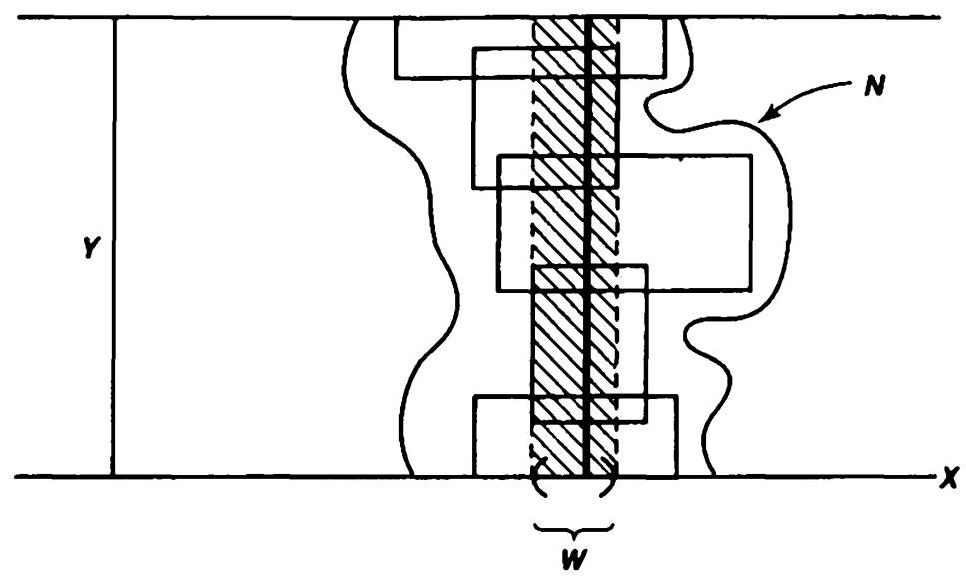
\includegraphics[width=0.8\textwidth]{images/26.2.jpg}
\end{center}
\hspace*{3em} 

Figure 26.2

Thus, for each \(x\) in \(X\) , we can choose a neighborhood \({W}_{x}\) of \(x\) such that the tube \({W}_{x} \times Y\) can be covered by finitely many elements of \(\mathcal{A}\) . The collection of all the neighborhoods \({W}_{x}\) is an open covering of \(X\) ; therefore by compactness of \(X\) , there exists a finite subcollection

\[
\left\{ {{W}_{1},\ldots,{W}_{k}}\right\}
\]

covering \(X\) . The union of the tubes

\[
{W}_{1} \times Y,\ldots,{W}_{k} \times Y
\]

is all of \(X \times Y\) ; since each may be covered by finitely many elements of \(\mathcal{A}\) , so may \(X \times Y\) be covered.

The statement proved in Step 1 of the preceding proof will be useful to us later, so we repeat it here as a lemma, for reference purposes:
\end{proof}

\begin{lemma}[The tube lemma] Consider the product space \(X \times Y\) , where \(Y\) is compact. If \(N\) is an open set of \(X \times Y\) containing the slice \({x}_{0} \times Y\) of \(X \times Y\) , then \(N\) contains some tube \(W \times Y\) about \({x}_{0} \times Y\) , where \(W\) is a neighborhood of \({x}_{0}\) in \(X\) .
\end{lemma}

\begin{centeredblock}
\begin{example} The tube lemma is certainly not true if \(Y\) is not compact For example, let \(Y\) be the \(y\) -axis in \({\mathbb{R}}^{2}\) , and let

\[
N = \left\{ {x \times y,\left| x\right| < 1/\left( {{y}^{2} + 1}\right) }\right\} .
\]

Then \(N\) is an open set containing the set \(0 \times \mathbb{R}\) , but it contains no tube about \(0 \times \mathbb{R}\) It is illustrated in Figure 263

\begin{center}
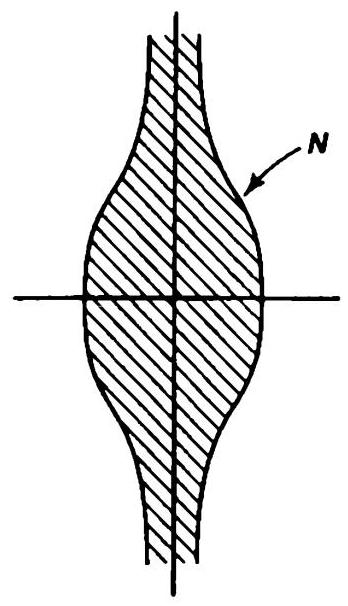
\includegraphics[width=0.3\textwidth]{images/26.3.jpg}
\end{center}
\hspace*{3em}

Figure 26.3
\end{example}
\end{centeredblock}

There is an obvious question to ask at this point. Is the product of infinitely many compact spaces compact? One would hope that the answer is ``yes,'' and in fact it is. The result is important (and difficult) enough to be called by the name of the man who proved it; it is called the Tychonoff theorem

In proving the fact that a cartesian product of connected spaces is connected, one proves it first for finite products and derives the general case from that. In proving that cartesian products of compact spaces are compact, however, there is no way to go directly from finite products to infinite ones. The infinite case demands a new approach, and the proof is a difficult one. Because of its difficulty, and also to avoid losing the main thread of our discussion in this chapter, we have decided to postpone it until later. However, you can study it now if you wish; the section in which it is proved (§37) can be studied immediately after this section without causing any disruption in continuity.

There is one final criterion for a space to be compact, a criterion that is formulated in terms of closed sets rather than open sets It does not look very natural nor very useful at first glance, but it in fact proves to be useful on a number of occasions. First we make a definition.

\begin{definition} A collection \(\mathcal{C}\) of subsets of \(X\) is said to have the finite intersection property if for every finite subcollection

\[
\left\{ {{C}_{1},\ldots,{C}_{n}}\right\}
\]

of \(\mathcal{C}\) , the intersection \({C}_{1} \cap \cdots \cap {C}_{n}\) is nonempty.
\end{definition}

\begin{theorem} Let \(X\) be a topological space. Then \(X\) is compact if and only if for every collection \(\mathcal{C}\) of closed sets in \(X\) having the finite intersection property, the intersection \(\mathop{\bigcap }\limits_{{C \in \mathcal{C}}}C\) of all the elements of \(\mathcal{C}\) is nonempty.
\end{theorem}
\begin{proof}Given a collection \(\mathcal{A}\) of subsets of \(X\) , let

\[
\mathcal{C} = \{ X - A \mid A \in \mathcal{A}\}
\]

be the collection of their complements. Then the following statements hold:

(I) \(\mathcal{A}\) is a collection of open sets if and only if \(\mathcal{C}\) is a collection of closed sets.

(2) The collection \(\mathcal{A}\) covers \(X\) if and only if the intersection \(\mathop{\bigcap }\limits_{{C \in \mathcal{C}}}C\) of all the elements of \(C\) is empty

(3) The finite subcollection \(\left\{ {{A}_{1},\ldots,{A}_{n}}\right\}\) of \(\mathcal{A}\) covers \(X\) if and only if the intersection of the corresponding elements \({C}_{l} = X - {A}_{i}\) of \(\mathcal{C}\) is empty.

The first statement is trivial, while the second and third follow from DeMorgan's law:

\[
X - \left( {\mathop{\bigcup }\limits_{{\alpha \in J}}{A}_{\alpha }}\right) = \mathop{\bigcap }\limits_{{\alpha \in J}}\left( {X - {A}_{\alpha }}\right)
\]

The proof of the theorem now proceeds in two easy steps: taking the contrapositive (of the theorem), and then the complement (of the sets)!

The statement that \(X\) is compact is equivalent to saying: ``Given any collection \(\mathcal{A}\) of open subsets of \(X\) , if \(\mathcal{A}\) covers \(X\) , then some finite subcollection of \(\mathcal{A}\) covers \(X\) .'' This statement is equivalent to its contrapositive, which is the following: ``Given any collection \(\mathcal{A}\) of open sets, if no finite subcollection of \(\mathcal{A}\) covers \(X\) , then \(\mathcal{A}\) does not cover \(X\) .'' Letting \(\mathcal{C}\) be, as earlier, the collection \(\{ X - A \mid A \in \mathcal{A}\}\) and applying (1)-(3), we see that this statement is in turn equivalent to the following: ``Given any collection \(\mathcal{C}\) of closed sets, if every finite intersection of elements of \(\mathcal{C}\) is nonempty, then the intersection of all the elements of \(\mathcal{C}\) is nonempty.'' This is just the condition of our theorem.

A special case of this theorem occurs when we have a nested sequence \({C}_{1} \supset {C}_{2} \supset\) \(\cdots \supset {C}_{n} \supset {C}_{n + 1} \supset \ldots\) of closed sets in a compact space \(X\) . If each of the sets \({C}_{n}\) is nonempty, then the collection \(\mathcal{C} = {\left\{ {C}_{n}\right\} }_{n \in {\mathbf{Z}}_{ + }}\) automatically has the finite intersection property. Then the intersection

\[
\mathop{\bigcap }\limits_{{n \in {\mathbf{Z}}_{ + }}}{C}_{n}
\]

is nonempty.

We shall use the closed set criterion for compactness in the next section to prove the uncountability of the set of real numbers, in Chapter 5 when we prove the Ty-chonoff theorem, and again in Chapter 8 when we prove the Baire category theorem.

\end{proof}
\section*{Exercises}

1. (a) Let \(\mathcal{T}\) and \({\mathcal{T}}^{\prime }\) be two topologies on the set \(X\) ; suppose that \({\mathcal{T}}^{\prime } \supset \mathcal{T}\) . What does compactness of \(X\) under one of these topologies imply about compactness under the other?

(b) Show that if \(X\) is compact Hausdorff under both \(\mathcal{T}\) and \({\mathcal{T}}^{\prime }\) , then either \(\mathcal{T}\) and \({\mathcal{T}}^{\prime }\) are equal or they are not comparable.

2. (a) Show that in the finite complement topology on \(\mathbb{R}\) , every subspace is compact.

(b) If \(\mathbb{R}\) has the topology consisting of all sets \(A\) such that \(\mathbb{R} - A\) is either countable or all of \(\mathbb{R}\) , is \(\left\lbrack {0,1}\right\rbrack\) a compact subspace?

3. Show that a finite union of compact subspaces of \(X\) is compact.

4. Show that every compact subspace of a metric space is bounded in that metric and is closed. Find a metric space in which not every closed bounded subspace is compact.

5. Let \(A\) and \(B\) be disjoint compact subspaces of the Hausdorff space \(X\) . Show that there exist disjoint open sets \(U\) and \(V\) containing \(A\) and \(B\) , respectively.

6. Show that if \(f: X \rightarrow Y\) is continuous, where \(X\) is compact and \(Y\) is Hausdorff, then \(f\) is a closed map (that is, \(f\) carries closed sets to closed sets).

7. Show that if \(Y\) is compact, then the projection \({\pi }_{1} : X \times Y \rightarrow X\) is a closed map.

8. Theorem. Let \(f: X \rightarrow Y\) ; let \(Y\) be compact Hausdorff. Then \(f\) is continuous if and only if the graph of \(f\) ,

\[
{G}_{f} = \{ x \times f\left( x\right) \mid x \in X\}
\]

is closed in \(X \times Y\) . [Hint: If \({G}_{f}\) is closed and \(V\) is a neighborhood of \(f\left( {x}_{0}\right)\) , then the intersection of \({G}_{f}\) and \(X \times \left( {Y - V}\right)\) is closed. Apply Exercise 7.]

9. Generalize the tube lemma as follows:

\begin{theorem} Let \(A\) and \(B\) be subspaces of \(X\) and \(Y\) , respectively; let \(N\) be an open set in \(X \times Y\) containing \(A \times B\) . If \(A\) and \(B\) are compact, then there exist open sets \(U\) and \(V\) in \(X\) and \(Y\) , respectively, such that

\[
A \times B \subset U \times V \subset N.
\]

10. (a) Prove the following partial converse to the uniform limit theorem:

\end{theorem}
\begin{theorem} Let \({f}_{n} : X \rightarrow \mathbb{R}\) be a sequence of continuous functions, with \({f}_{n}\left( x\right) \rightarrow f\left( x\right)\) for each \(x \in X\) . If \(f\) is continuous, and if the sequence \({f}_{n}\) is monotone increasing, and if \(X\) is compact, then the convergence is uniform. [We say that \({f}_{n}\) is monotone increasing if \({f}_{n}\left( x\right) \leq {f}_{n + 1}\left( x\right)\) for all \(n\) and \(x\) .]

(b) Give examples to show that this theorem fails if you delete the requirement that \(X\) be compact, or if you delete the requirement that the sequence be monotone. [Hint: See the exercises of §21.]

11. Theorem. Let \(X\) be a compact Hausdorff space. Let \(\mathcal{A}\) be a collection of closed connected subsets of \(X\) that is simply ordered by proper inclusion. Then

\[
Y = \mathop{\bigcap }\limits_{{A \in \mathcal{A}}}A
\]

is connected. [Hint: If \(C \cup D\) is a separation of \(Y\) , choose disjoint open sets \(U\) and \(V\) of \(X\) containing \(C\) and \(D\) , respectively, and show that

\[
\mathop{\bigcap }\limits_{{A \in \mathcal{A}}}\left( {A - \left( {U \cup V}\right) }\right)
\]

is not empty.]

12. Let \(p: X \rightarrow Y\) be a closed continuous surjective map such that \({p}^{-1}\left( {\{ y\} }\right)\) is compact, for each \(y \in Y\) . (Such a map is called a perfect map ) Show that if \(Y\) is compact, then \(X\) is compact. [Hint: If \(U\) is an open set containing \({p}^{-1}\left( {\{ y\} }\right)\) , there is a neighborhood \(W\) of \(y\) such that \({p}^{-1}\left( W\right)\) is contained in \(U\) ]

13. Let \(G\) be a topological group.

(a) Let \(A\) and \(B\) be subspaces of \(G\) . If \(A\) is closed and \(B\) is compact, show \(A \cdot B\) is closed. [Hint: If \(c\) is not in \(A \cdot B\) , find a neighborhood \(W\) of \(c\) such that \(W \cdot {B}^{-1}\) is disjoint from \(A\) .]

(b) Let \(H\) be a subgroup of \(G\) ; let \(p \cdot G \rightarrow G/H\) be the quotient map. If \(H\) is compact, show that \(p\) is a closed map.

(c) Let \(H\) be a compact subgroup of \(G\) . Show that if \(G/H\) is compact, then \(G\) is compact.

\end{theorem}
\section*{§ 27 Compact Subspaces of the Real Line}

The theorems of the preceding section enable us to construct new compact spaces from existing ones, but in order to get very far we have to find some compact spaces to start with. The natural place to begin is the real line; we shall prove that every closed interval in \(\mathbb{R}\) is compact. Applications include the extreme value theorem and the uniform continuity theorem of calculus, suitably generalized. We also give a characterization of all compact subspaces of \({\mathbb{R}}^{n}\) , and a proof of the uncountability of the set of real numbers.

It turns out that in order to prove every closed interval in \(\mathbb{R}\) is compact, we need only one of the order properties of the real line-the least upper bound property. We shall prove the theorem using only this hypothesis; then it will apply not only to the real line, but to well-ordered sets and other ordered sets as well.

\begin{theorem} Let \(X\) be a simply ordered set having the least upper bound property. In the order topology, each closed interval in \(X\) is compact.

\end{theorem}
\begin{proof}
Step 1. Given \(a < b\) , let \(\mathcal{A}\) be a covering of \(\left\lbrack {a,b}\right\rbrack\) by sets open in \(\left\lbrack {a,b}\right\rbrack\) in the subspace topology (which is the same as the order topology). We wish to prove the existence of a finite subcollection of \(\mathcal{A}\) covering \(\left\lbrack {a,b}\right\rbrack\) . First we prove the following: If \(x\) is a point of \(\left\lbrack {a,b}\right\rbrack\) different from \(b\) , then there is a point \(y > x\) of \(\left\lbrack {a,b}\right\rbrack\) such that the interval \(\left\lbrack {x,y}\right\rbrack\) can be covered by at most two elements of \(\mathcal{A}\)

If \(x\) has an immediate successor in \(X\) , let \(y\) be this immediate successor. Then \(\left\lbrack {x,y}\right\rbrack\) consists of the two points \(x\) and \(y\) , so that it can be covered by at most two elements of \(\mathcal{A}\) . If \(x\) has no immediate successor in \(X\) , choose an element \(A\) of \(\mathcal{A}\) containing \(x\) . Because \(x \neq b\) and \(A\) is open, \(A\) contains an interval of the form \(\lbrack x,c)\) , for some \(c\) in \(\left\lbrack {a,b}\right\rbrack\) . Choose a point \(y\) in(x, c); then the interval \(\left\lbrack {x,y}\right\rbrack\) is covered by the single element \(A\) of \(\mathcal{A}\) .

Step 2. Let \(C\) be the set of all points \(y > a\) of \(\left\lbrack {a,b}\right\rbrack\) such that the interval \(\left\lbrack {a,y}\right\rbrack\) can be covered by finitely many elements of \(\mathcal{A}\) Applying Step 1 to the case \(x = a\) , we see that there exists at least one such \(y\) , so \(C\) is not empty. Let \(c\) be the least upper bound of the set \(C\) ; then \(a < c \leq b\) .

Step 3. We show that \(c\) belongs to \(C\) ; that is, we show that the interval \(\left\lbrack {a,c}\right\rbrack\) can be covered by finitely many elements of \(\mathcal{A}\) . Choose an element \(A\) of \(\mathcal{A}\) containing \(c\) ; since \(A\) is open, it contains an interval of the form \((d,c\rbrack\) for some \(d\) in \(\left\lbrack {a,b}\right\rbrack\) . If \(c\) is not in \(C\) , there must be a point \(z\) of \(C\) lying in the interval(d, c), because otherwise \(d\) would be a smaller upper bound on \(C\) than \(c\) . See Figure 27.1. Since \(z\) is in \(C\) , the interval \(\left\lbrack {a,z}\right\rbrack\) can be covered by finitely many, say \(n\) , elements of \(\mathcal{A}\) . Now \(\left\lbrack {z,c}\right\rbrack\) lies in the single element \(A\) of \(\mathcal{A}\) , hence \(\left\lbrack {a,c}\right\rbrack = \left\lbrack {a,z}\right\rbrack \cup \left\lbrack {z,c}\right\rbrack\) can be covered by \(n + 1\) elements of \(\mathcal{A}\) . Thus \(c\) is in \(C\) , contrary to assumption.

\begin{center}
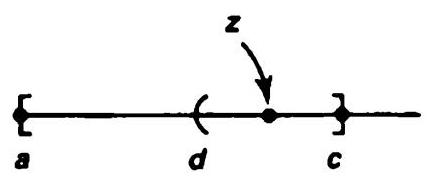
\includegraphics[width=0.4\textwidth]{images/27.1.jpg}
\end{center}
\hspace*{3em} 

Figure 27.1

\begin{center}
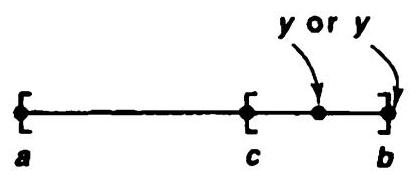
\includegraphics[width=0.3\textwidth]{images/27.2.jpg}
\end{center}
\hspace*{3em} 

Figure 27.2

Step 4. Finally, we show that \(c = b\) , and our theorem is proved. Suppose that \(c < b\) . Applying Step 1 to the case \(x = c\) , we conclude that there exists a point \(y > c\) of \(\left\lbrack {a,b}\right\rbrack\) such that the interval \(\left\lbrack {c,y}\right\rbrack\) can be covered by finitely many elements of \(\mathcal{A}\) . See Figure 27.2. We proved in Step 3 that \(c\) is in \(C\) , so \(\left\lbrack {a,c}\right\rbrack\) can be covered by finitely many elements of \(\mathcal{A}\) . Therefore, the interval

\[
\left\lbrack {a,y}\right\rbrack = \left\lbrack {a,c}\right\rbrack \cup \left\lbrack {c,y}\right\rbrack
\]

can also be covered by finitely many elements of \(\mathcal{A}\) . This means that \(y\) is in \(C\) , contradicting the fact that \(c\) is an upper bound on \(C\) .
\end{proof}

\begin{corollary} Every closed interval in \(\mathbb{R}\) is compact.
\end{corollary}

Now we charactenze the compact subspaces of \({\mathbb{R}}^{n}\) :

\begin{theorem} A subspace \(A\) of \({\mathbb{R}}^{n}\) is compact if and only if it is closed and is bounded in the euclidean metric \(d\) or the square metric \(\rho\) .

\end{theorem}
\begin{proof}
It will suffice to consider only the metric \(\rho\) ; the inequalities

\[
\rho \left( {x,y}\right) \leq d\left( {x,y}\right) \leq \sqrt{n}\rho \left( {x,y}\right)
\]

imply that \(A\) is bounded under \(d\) if and only if it is bounded under \(\rho\) .

Suppose that \(A\) is compact. Then, by Theorem 26.3, it is closed. Consider the collection of open sets

\[
\left\{ {{B}_{\rho }\left( {0,m}\right) \mid m \in {\mathbb{Z}}_{ + }}\right\} ,
\]

whose union is all of \({\mathbb{R}}^{n}\) . Some finite subcollection covers \(A\) It follows that \(A \subset\) \({B}_{\rho }\left( {0,M}\right)\) for some \(M\) . Therefore, for any two points \(x\) and \(y\) of \(A\) , we have \(\rho \left( {x,y}\right) \leq\) \({2M}\) . Thus \(A\) is bounded under \(\rho\) .

Conversely, suppose that \(A\) is closed and bounded under \(\rho\) ; suppose that \(\rho \left( {x,y}\right) \leq\) \(N\) for every pair \(x,y\) of points of \(A\) . Choose a point \({x}_{0}\) of \(A\) , and let \(\rho \left( {{x}_{0},\mathbf{0}}\right) = b\) . The triangle inequality implies that \(\rho \left( {x,\mathbf{0}}\right) \leq N + b\) for every \(x\) in \(A\) . If \(P = N + b\) , then \(A\) is a subset of the cube \(\{ - P,P{\} }^{n}\) , which is compact. Being closed, \(A\) is also compact.

Students often remember this theorem as stating that the collection of compact sets in a metric space equals the collection of closed and bounded sets. This statement is clearly ridiculous as it stands, because the question as to which sets are bounded depends for its answer on the metric, whereas which sets are compact depends only on the topology of the space.
\end{proof}

\begin{centeredblock}
\begin{example} The unit sphere \({S}^{n - 1}\) and the closed unit ball \({B}^{n}\) in \({\mathbb{R}}^{n}\) are compact because they are closed and bounded. The set

\[
A = \{ x \times \left( {1/x}\right) \mid 0 < x \leq 1\}
\]

is closed in \({\mathbf{R}}^{2}\) , but it is not compact because it is not bounded. The set

\[
S = \{ x \times \left( {\sin \left( {1/x}\right) }\right) \mid 0 < x \leq 1\}
\]

is bounded in \({\mathbb{R}}^{2}\) , but it is not compact because it is not closed
\end{example}
\end{centeredblock}

Now we prove the extreme value theorem of calculus, in suitably generalized form.

\begin{theorem}[Extreme value theorem] Let \(f: X \rightarrow Y\) be continuous, where \(Y\) is an ordered set in the order topology. If \(X\) is compact, then there exist points \(c\) and \(d\) in \(X\) such that \(f\left( c\right) \leq f\left( x\right) \leq f\left( d\right)\) for every \(x \in X\) .

The extreme value theorem of calculus is the special case of this theorem that occurs when we take \(X\) to be a closed interval in \(\mathbb{R}\) and \(Y\) to be \(\mathbb{R}\) .

\end{theorem}
\begin{proof}
Since \(f\) is continuous and \(X\) is compact, the set \(A = f\left( X\right)\) is compact. We show that \(A\) has a largest element \(M\) and a smallest element \(m\) . Then since \(m\) and \(M\) belong to \(A\) , we must have \(m = f\left( c\right)\) and \(M = f\left( d\right)\) for some points \(c\) and \(d\) of \(X\) .

If \(A\) has no largest element, then the collection

\[
\{ \left( {-\infty,a}\right) \mid a \in A\}
\]

forms an open covering of \(A\) . Since \(A\) is compact, some finite subcollection

\[
\left\{ {\left( {-\infty,{a}_{1}}\right) ,\ldots,\left( {-\infty,{a}_{n}}\right) }\right\}
\]

covers \(A\) If \({a}_{i}\) is the largest of the elements \({a}_{1},\ldots {a}_{n}\) , then \({a}_{i}\) belongs to none of these sets, contrary to the fact that they cover \(A\) .

A similar argument shows that \(A\) has a smallest element.

Now we prove the uniform continuity theorem of calculus. In the process, we are led to introduce a new notion that will prove to be surprisingly useful, that of a Lebesgue number for an open covering of a metric space. First, a preliminary notion:
\end{proof}

\begin{definition} Let(X, d)be a metric space; let \(A\) be a nonempty subset of \(X\) . For each \(x \in X\) , we define the distance from \(x\) to \(A\) by the equation

\[
d\left( {x,A}\right) = \inf \{ d\left( {x,a}\right) \mid a \in A\} .
\]
\end{definition}

It is easy to show that for fixed \(A\) , the function \(d\left( {x,A}\right)\) is a continuous function of \(x\) : Given \(x,y \in X\) , one has the inequalities

\[
d\left( {x,A}\right) \leq d\left( {x,a}\right) \leq d\left( {x,y}\right) + d\left( {y,a}\right) ,
\]

for each \(a \in A\) . It follows that

\[
d\left( {x,A}\right) - d\left( {x,y}\right) \leq \inf d\left( {y,a}\right) = d\left( {y,A}\right) ,
\]

so that

\[
d\left( {x,A}\right) - d\left( {y,A}\right) \leq d\left( {x,y}\right) .
\]

The same inequality holds with \(x\) and \(y\) interchanged; continuity of the function \(d\left( {x,A}\right)\) follows.

Now we introduce the notion of Lebesgue number. Recall that the diameter of a bounded subset \(A\) of a metric space(X, d)is the number

\[
\sup \left\{ {d\left( {{a}_{1},{a}_{2}}\right) \mid {a}_{1},{a}_{2} \in A}\right\} .
\]

\begin{lemma}[The Lebesgue number lemma] Let \(\mathcal{A}\) be an open covering of the metric space(X, d). If \(X\) is compact, there is a \(\delta > 0\) such that for each subset of \(X\) having diameter less than \(\delta\) , there exists an element of \(\mathcal{A}\) containing it.
\end{lemma}

The number \(\delta\) is called a Lebesgue number for the covering \(\mathcal{A}\) .

\begin{proof}
Let \(\mathcal{A}\) be an open covering of \(X\) . If \(X\) itself is an element of \(\mathcal{A}\) , then any positive number is a Lebesgue number for \(\mathcal{A}\) . So assume \(X\) is not an element of \(\mathcal{A}\) .

Choose a finite subcollection \(\left\{ {{A}_{1},\ldots,{A}_{n}}\right\}\) of \(\mathcal{A}\) that covers \(X\) . For each \(i\) , set \({C}_{i} = X - {A}_{i}\) , and define \(f: X \rightarrow \mathbb{R}\) by letting \(f\left( x\right)\) be the average of the numbers \(d\left( {x,{C}_{l}}\right)\) . That is,

\[
f\left( x\right) = \frac{1}{n}\mathop{\sum }\limits_{{i = 1}}^{n}d\left( {x,{C}_{i}}\right) .
\]

We show that \(f\left( x\right) > 0\) for all \(x\) . Given \(x \in X\) , choose \(i\) so that \(x \in {A}_{i}\) . Then choose \(\epsilon\) so the \(\epsilon\) -neighborhood of \(x\) lies in \({A}_{i}\) . Then \(d\left( {x,{C}_{i}}\right) \geq \epsilon\) , so that \(f\left( x\right) \geq \epsilon /n\) .

Since \(f\) is continuous, it has a minimum value \(\delta\) ; we show that \(\delta\) is our required Lebesgue number Let \(B\) be a subset of \(X\) of diameter less than \(\delta\) . Choose a point \({x}_{0}\) of \(B\) , then \(B\) lies in the \(\delta\) -neighborhood of \({x}_{0}\) . Now

\[
\delta \leq f\left( {x}_{0}\right) \leq d\left( {{x}_{0},{C}_{m}}\right)
\]

where \(d\left( {{x}_{0},{C}_{m}}\right)\) is the largest of the numbers \(d\left( {{x}_{0},{C}_{l}}\right)\) . Then the \(\delta\) -neighborhood of \({x}_{0}\) is contained in the element \({A}_{m} = X - {C}_{m}\) of the covering \(\mathcal{A}\) .
\end{proof}

\begin{definition} A function \(f\) from the metric space \(\left( {X,{d}_{X}}\right)\) to the metric space \(\left( {Y,{d}_{Y}}\right)\) is said to be uniformly continuous if given \(\epsilon > 0\) , there is a \(\delta > 0\) such that for every pair of points \({x}_{0},{x}_{1}\) of \(X\) ,

\[
{d}_{X}\left( {{x}_{0},{x}_{1}}\right) < \delta \Rightarrow {d}_{Y}\left( {f\left( {x}_{0}\right) ,f\left( {x}_{1}\right) }\right) < \epsilon
\]
\end{definition}

\begin{theorem}[Uniform continuity theorem] Let \(f: X \rightarrow Y\) be a continuous map of the compact metric space \(\left( {X,{d}_{X}}\right)\) to the metric space \(\left( {Y,{d}_{Y}}\right)\) . Then \(f\) is uniformly continuous.

\end{theorem}
\begin{proof}
Given \(\epsilon > 0\) , take the open covering of \(Y\) by balls \(B\left( {y,\epsilon /2}\right)\) of radius \(\epsilon /2\) . Let \(\mathcal{A}\) be the open covering of \(X\) by the inverse images of these balls under \(f\) . Choose \(\delta\) to be a Lebesgue number for the covering \(\mathcal{A}\) . Then if \({x}_{1}\) and \({x}_{2}\) are two points of \(X\) such that \({d}_{\chi }\left( {{x}_{1},{x}_{2}}\right) < \delta\) , the two-point set \(\left\{ {{x}_{1},{x}_{2}}\right\}\) has diameter less than \(\delta\) , so that its image \(\left\{ {f\left( {x}_{1}\right) ,f\left( {x}_{2}\right) }\right\}\) lies in some ball \(B\left( {y,\epsilon /2}\right)\) . Then \({d}_{Y}\left( {f\left( {x}_{1}\right) ,f\left( {x}_{2}\right) }\right) < \epsilon\) , as desired

Finally, we prove that the real numbers are uncountable. The interesting thing about this proof is that it involves no algebra at all-no decimal or binary expansions of real numbers or the like-just the order properties of \(\mathbb{R}\) .
\end{proof}

\begin{definition} If \(X\) is a space, a point \(x\) of \(X\) is said to be an isolated point of \(X\) if the one-point set \(\{ x\}\) is open in \(X\)
\end{definition}

\begin{theorem} Let \(X\) be a nonempty compact Hausdorff space. If \(X\) has no isolated points, then \(X\) is uncountable.

\end{theorem}
\begin{proof}
Step 1. We show first that given any nonempty open set \(U\) of \(X\) and any point \(x\) of \(X\) , there exists a nonempty open set \(V\) contained in \(U\) such that \(x \notin \bar{V}\)

Choose a point \(y\) of \(U\) different from \(x\) ; this is possible if \(x\) is in \(U\) because \(x\) is not an isolated point of \(X\) and it is possible if \(x\) is not in \(U\) simply because \(U\) is nonempty. Now choose disjoint open sets \({W}_{1}\) and \({W}_{2}\) about \(x\) and \(y\) , respectively. Then the set \(V = {W}_{2} \cap U\) is the desired open set, it is contained in \(U\) , it is nonempty because it contains \(y\) , and its closure does not contain \(x\) See Figure 27.3

Step 2. We show that given \(f: {\mathbb{Z}}_{ + } \rightarrow X\) , the function \(f\) is not surjective. It follows that \(X\) is uncountable

\begin{center}
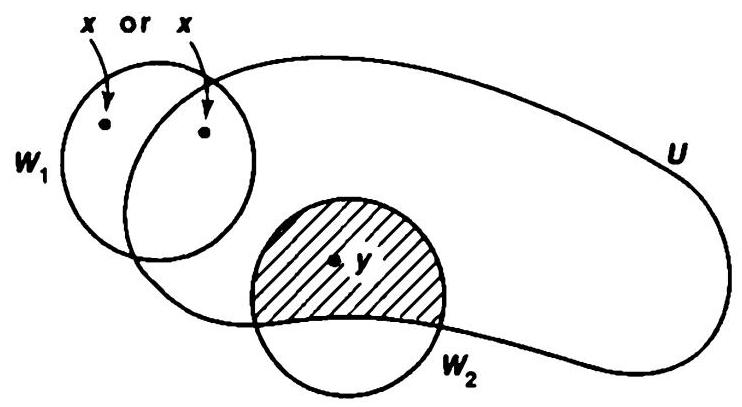
\includegraphics[width=0.6\textwidth]{images/27.3.jpg}
\end{center}
\hspace*{3em} 

Figure 27.3

Let \({x}_{n} = f\left( n\right)\) . Apply Step 1 to the nonempty open set \(U = X\) to choose a nonempty open set \({V}_{1} \subset X\) such that \({\bar{V}}_{1}\) does not contain \({x}_{1}\) . In general, given \({V}_{n - 1}\) open and nonempty, choose \({V}_{n}\) to be a nonempty open set such that \({V}_{n} \subset {V}_{n - 1}\) and \({\bar{V}}_{n}\) does not contain \({x}_{n}\) . Consider the nested sequence

\[
{\bar{V}}_{1} \supset {\bar{V}}_{2} \supset \cdots
\]

of nonempty closed sets of \(X\) . Because \(X\) is compact, there is a point \(x \in \bigcap {\bar{V}}_{n}\) , by Theorem 26.9. Now \(x\) cannot equal \({x}_{n}\) for any \(n\) , since \(x\) belongs to \({V}_{n}\) and \({x}_{n}\) does not.
\end{proof}

\begin{corollary} Every closed interval in \(\mathbb{R}\) is uncountable.
\end{corollary}

\section*{Exercises}

1. Prove that if \(X\) is an ordered set in which every closed interval is compact, then \(X\) has the least upper bound property.

2. Let \(X\) be a metric space with metric \(d\) ; let \(A \subset X\) be nonempty.

(a) Show that \(d\left( {x,A}\right) = 0\) if and only if \(x \in \bar{A}\) .

(b) Show that if \(A\) is compact, \(d\left( {x,A}\right) = d\left( {x,a}\right)\) for some \(a \in A\) .

(c) Define the \(\epsilon\) -neighborhood of \(A\) in \(X\) to be the set

\[
U\left( {A,\epsilon }\right) = \{ x \mid d\left( {x,A}\right) < \epsilon \} .
\]

Show that \(U\left( {A,\epsilon }\right)\) equals the union of the open balls \({B}_{d}\left( {a,\epsilon }\right)\) for \(a \in A\)

(d) Assume that \(A\) is compact; let \(U\) be an open set containing \(A\) . Show that some \(\epsilon\) -neighborhood of \(A\) is contained in \(U\) .

(e) Show the result in (d) need not hold if \(A\) is closed but not compact.

3. Recall that \({\mathbb{R}}_{K}\) denotes \(\mathbb{R}\) in the \(K\) -topology.

(a) Show that \(\left\lbrack {0,1}\right\rbrack\) is not compact as a subspace of \({\mathbb{R}}_{K}\) .

(b) Show that \({\mathbb{R}}_{K}\) is connected. [Hint \(\left( {-\infty,0}\right)\) and \(\left( {0,\infty }\right)\) inherit their usual topologies as subspaces of \({\mathbb{R}}_{K}\) .]

(c) Show that \({\mathbb{R}}_{K}\) is not path connected.

4. Show that a connected metric space having more than one point is uncountable.

5. Let \(X\) be a compact Hausdorff space, let \(\left\{ {A}_{n}\right\}\) be a countable collection of closed sets of \(X\) . Show that if each set \({A}_{n}\) has empty interior in \(X\) , then the union \(\cup {A}_{n}\) has empty interior in \(X\) . [Hint: Imitate the proof of Theorem 27.7.]

This is a special case of the Baire category theorem, which we shall study in Chapter 8.

6. Let \({A}_{0}\) be the closed interval \(\left\lbrack {0,1}\right\rbrack\) in \(\mathbb{R}\) . Let \({A}_{1}\) be the set obtained from \({A}_{0}\) by deleting its ``middle third'' \(\left( {\frac{1}{3},\frac{2}{3}}\right)\) . Let \({A}_{2}\) be the set obtained from \({A}_{1}\) by deleting its ``middle thirds'' \(\left( {\frac{1}{9},\frac{2}{9}}\right)\) and \(\left( {\frac{7}{9},\frac{8}{9}}\right)\) In general, define \({A}_{n}\) by the equation

\[
{A}_{n} = {A}_{n - 1} - \mathop{\bigcup }\limits_{{k = 0}}^{\infty }\left( {\frac{1 + {3k}}{{3}^{n}},\frac{2 + {3k}}{{3}^{n}}}\right) .
\]

The intersection

\[
C = \mathop{\bigcap }\limits_{{n \in {\mathbf{Z}}_{ + }}}{A}_{n}
\]

is called the Cantor set; it is a subspace of \(\left\lbrack {0,1}\right\rbrack\)

(a) Show that \(C\) is totally disconnected.

(b) Show that \(C\) is compact.

(c) Show that each set \({A}_{n}\) is a union of finitely many disjoint closed intervals of length \(1/{3}^{n}\) ; and show that the end points of these intervals lie in \(C\) .

(d) Show that \(C\) has no isolated points.

(e) Conclude that \(C\) is uncountable.

\section*{§ 28 Limit Point Compactness}

As indicated when we first mentioned compact sets, there are other formulations of the notion of compactness that are frequently useful. In this section we introduce one of them. Weaker in general than compactness, it coincides with compactness for metrizable spaces.

\begin{definition} A space \(X\) is said to be limit point compact if every infinite subset of \(X\) has a limit point.
\end{definition}

In some ways this property is more natural and intuitive than that of compactness. In the early days of topology, it was given the name ``compactness,'' while the open covering formulation was called ``bicompactness.'' Later, the word ``compact'' was shifted to apply to the open covering definition, leaving this one to search for a new name It still has not found a name on which everyone agrees On historical grounds, some call it ``Fréchet compactness'', others call it the ``Bolzano-Weierstrass property'' We have invented the term ``limit point compactness'' It seems as good a term as any; at least it describes what the property is about.

\section*{Theorem 28.1. Compactness implies limit point compactness, but not con versely}

\begin{proof}
Let \(X\) be a compact space. Given a subset \(A\) of \(X\) , we wish to prove that if \(A\) is infinite, then \(A\) has a limit point. We prove the contrapositive-if \(A\) has no limit point, then \(A\) must be finite.

So suppose \(A\) has no limit point. Then \(A\) contains all its limit points, so that \(A\) is closed. Furthermore, for each \(a \in A\) we can choose a neighborhood \({U}_{a}\) of \(a\) such that \({U}_{a}\) intersects \(A\) in the point \(a\) alone The space \(X\) is covered by the open set \(X - A\) and the open sets \({U}_{a}\) ; being compact, it can be covered by finitely many of these sets. Since \(X - A\) does not intersect \(A\) , and each set \({U}_{a}\) contains only one point of \(A\) , the set \(A\) must be finite.
\end{proof}

\begin{centeredblock}
\begin{example} Let \(Y\) consist of two points, give \(Y\) the topology consisting of \(Y\) and the empty set Then the space \(X = {\mathbb{Z}}_{ + } \times Y\) is limit point compact, for every nonempty subset of \(X\) has a limit point. It is not compact, for the covering of \(X\) by the open sets \({U}_{n} = \left\lbrack n\right\rbrack \times Y\) has no finite subcollection covering \(X\)
\end{example}
\end{centeredblock}

\begin{centeredblock}
\begin{example} Here is a less trivial example Consider the minimal uncountable well-ordered set \({S}_{\Omega }\) , in the order topology The space \({S}_{\Omega }\) is not compact, since it has no largest element However, it is limit point compact Let \(A\) be an infinite subset of \({S}_{\Omega }\) . Choose a subset \(B\) of \(A\) that is countably infinite Being countable, the set \(B\) has an upper bound \(b\) in \({S}_{\Omega }\) ; then \(B\) is a subset of the interval \(\left\lbrack {{a}_{0},b}\right\rbrack\) of \({S}_{\Omega }\) , where \({a}_{0}\) is the smallest element of \({S}_{\Omega }\) . Since \({S}_{\Omega }\) has the least upper bound property, the interval \(\left\lbrack {{a}_{0},b}\right\rbrack\) is compact By the preceding theorem, \(B\) has a limit point \(x\) in \(\left\lbrack {{a}_{0},b}\right\rbrack\) . The point \(x\) is also a limit point of \(A\) Thus \({S}_{\Omega }\) is limit point compact
\end{example}
\end{centeredblock}

We now show these two versions of compactness coincide for metrizable spaces; for this purpose, we introduce yet another version of compactness called sequential compactness. This result will be used in Chapter 7.

\begin{definition} Let \(X\) be a topological space. If \(\left( {x}_{n}\right)\) is a sequence of points of \(X\) , and if

\[
{n}_{1} < {n}_{2} < \cdots < {n}_{i} < \cdots
\]

is an increasing sequence of positive integers, then the sequence \(\left( {y}_{i}\right)\) defined by setting \({y}_{i} = {x}_{{n}_{i}}\) is called a subsequence of the sequence \(\left( {x}_{n}\right)\) . The space \(X\) is said to be sequentially compact if every sequence of points of \(X\) has a convergent subsequence.
\end{definition}

*Theorem 28.2. Let \(X\) be a metrizable space. Then the following are equivalent:

(1) \(X\) is compact.

(2) \(X\) is limit point compact.

(3) \(X\) is sequentially compact. Proof. We have already proved that (1) \(\Rightarrow\) (2). To show that (2) \(\Rightarrow\) (3), assume that \(X\) is limit point compact. Given a sequence \(\left( {x}_{n}\right)\) of points of \(X\) , consider the set \(A = \left\{ {{x}_{n} \mid n \in {\mathbb{Z}}_{ + }}\right\}\) . If the set \(A\) is finite, then there is a point \(x\) such that \(x = {x}_{n}\) for infinitely many values of \(n\) . In this case, the sequence \(\left( {x}_{n}\right)\) has a subsequence that is constant, and therefore converges trivially. On the other hand, if \(A\) is infinite, then \(A\) has a limit point \(x\) . We define a subsequence of \(\left( {x}_{n}\right)\) converging to \(x\) as follows: First choose \({n}_{1}\) so that

\[
{x}_{{n}_{1}} \in B\left( {x,1}\right) \text{ . }
\]

Then suppose that the positive integer \({n}_{i - 1}\) is given. Because the ball \(B\left( {x,1/i}\right)\) intersects \(A\) in infinitely many points, we can choose an index \({n}_{i} > {n}_{i - 1}\) such that

\[
{x}_{{n}_{i}} \in B\left( {x,1/\iota }\right) \text{ . }
\]

Then the subsequence \({x}_{{n}_{1}},{x}_{{n}_{2}},\ldots\) converges to \(x\) .

Finally, we show that \(\left( 3\right) \Rightarrow \left( 1\right)\) . This is the hardest part of the proof.

First, we show that if \(X\) is sequentially compact, then the Lebesgue number lemma holds for \(X\) . (This would follow from compactness, but compactness is what we are trying to prove!) Let \(\mathcal{A}\) be an open covering of \(X\) . We assume that there is no \(\delta > 0\) such that each set of diameter less than \(\delta\) has an element of \(\mathcal{A}\) containing it, and derive a contradiction.

Our assumption implies in particular that for each positive integer \(n\) , there exists a set of diameter less than \(1/n\) that is not contained in any element of \(\mathcal{A}\) ; let \({C}_{n}\) be such a set. Choose a point \({x}_{n} \in {C}_{n}\) , for each \(n\) . By hypothesis, some subsequence \(\left( {x}_{{n}_{i}}\right)\) of the sequence \(\left( {x}_{n}\right)\) converges, say to the point \(a\) . Now \(a\) belongs to some element \(A\) of the collection \(\mathcal{A}\) ; because \(A\) is open, we may choose an \(\epsilon > 0\) such that \(B\left( {a,\epsilon }\right) \subset A\) . If \(i\) is large enough that \(1/{n}_{i} < \epsilon /2\) , then the set \({C}_{{n}_{i}}\) lies in the \(\epsilon /2\) -neighborhood of \({x}_{{n}_{i}}\) ; if \(i\) is also chosen large enough that \(d\left( {{x}_{{n}_{i}},a}\right) < \epsilon /2\) , then \({C}_{{n}_{i}}\) lies in the \(\epsilon\) -neighborhood of \(a\) . But this means that \({C}_{{n}_{t}} \subset A\) , contrary to hypothesis.

Second, we show that if \(X\) is sequentially compact, then given \(\epsilon > 0\) , there exists a finite covering of \(X\) by open \(\epsilon\) -balls. Once again, we proceed by contradiction. Assume that there exists an \(\epsilon > 0\) such that \(X\) cannot be covered by finitely many \(\epsilon\) -balls. Construct a sequence of points \({x}_{n}\) of \(X\) as follows: First, choose \({x}_{1}\) to be any point of \(X\) . Noting that the ball \(B\left( {{x}_{1},\epsilon }\right)\) is not all of \(X\) (otherwise \(X\) could be covered by a single \(\epsilon\) -ball), choose \({x}_{2}\) to be a point of \(X\) not in \(B\left( {{x}_{1},\epsilon }\right)\) . In general, given \({x}_{1},\ldots,{x}_{n}\) , choose \({x}_{n + 1}\) to be a point not in the union

\[
B\left( {{x}_{1},\epsilon }\right) \cup \cdots \cup B\left( {{x}_{n},\epsilon }\right) ,
\]

using the fact that these balls do not cover \(X\) . Note that by construction \(d\left( {{x}_{n + 1},{x}_{i}}\right) \geq\) \(\epsilon\) for \(i = 1,\ldots,n\) . Therefore, the sequence \(\left( {x}_{n}\right)\) can have no convergent subsequence; in fact, any ball of radius \(\epsilon /2\) can contain \({x}_{n}\) for at most one value of \(n\) .

Finally, we show that if \(X\) is sequentially compact, then \(X\) is compact. Let \(\mathcal{A}\) be an open covering of \(X\) . Because \(X\) is sequentially compact, the open covering \(\mathcal{A}\) has a Lebesgue number \(\delta\) . Let \(\epsilon = \delta /3\) ; use sequential compactness of \(X\) to find a finite covering of \(X\) by open \(\epsilon\) -balls. Each of these balls has diameter at most \({2\delta }/3\) , so it lies in an element of \(\mathcal{A}\) . Choosing one such element of \(\mathcal{A}\) for each of these \(\epsilon\) -balls, we obtain a finite subcollection of \(\mathcal{A}\) that covers \(X\) .

\begin{centeredblock}
\begin{example} Recall that \({\bar{S}}_{\Omega }\) denotes the minimal uncountable well-ordered set \({S}_{\Omega }\) with the point \(\Omega\) adjoined. (In the order topology, \(\Omega\) is a limit point of \({S}_{\Omega }\) , which is why we introduced the notation \({\bar{S}}_{\Omega }\) for \({S}_{\Omega } \cup \{ \Omega \}\) , back in \(\$ {10})\) It is easy to see that the space \({\bar{S}}_{\Omega }\) is not metrizable, for it does not satisfy the sequence lemma: The point \(\Omega\) is a limit point of \({S}_{\Omega }\) , but it is not the limit of a sequence of points of \({S}_{\Omega }\) , for any sequence of points of \({S}_{\Omega }\) has an upper bound in \({S}_{\Omega }\) The space \({S}_{\Omega }\) , on the other hand, does satisfy the sequence lemma, as you can readily check Nevertheless, \({S}_{\Omega }\) is not metrizable, for it is limit point compact but not compact.
\end{example}
\end{centeredblock}

\section*{Exercises}

1. Give \({\left\lbrack 0,1\right\rbrack }^{\omega }\) the uniform topology. Find an infinite subset of this space that has no limit point

2. Show that \(\left\lbrack {0,1}\right\rbrack\) is not limit point compact as a subspace of \({\mathbb{R}}_{\ell }\) .

3. Let \(X\) be limit point compact.

(a) If \(f \cdot X \rightarrow Y\) is continuous, does it follow that \(f\left( X\right)\) is limit point compact?

(b) If \(A\) is a closed subset of \(X\) , does it follow that \(A\) is limit point compact?

(c) If \(X\) is a subspace of the Hausdorff space \(Z\) , does it follow that \(X\) is closed in \(Z\) ?

We comment that it is not in general true that the product of two limit point compact spaces is limit point compact, even if the Hausdorff condition is assumed. But the examples are fairly sophisticated. See \cite{SteenSeebach1970}, Example II2.

4. A space \(X\) is said to be countably compact if every countable open covering of \(X\) contains a finite subcollection that covers \(X\) . Show that for a \({T}_{1}\) space \(X\) , countable compactness is equivalent to limit point compactness. [Hint: If no finite subcollection of \({U}_{n}\) covers \(X\) , choose \({x}_{n} \notin {U}_{1} \cup \cdots \cup {U}_{n}\) , for each \(n\) .]

5. Show that \(X\) is countably compact if and only if every nested sequence \({C}_{1} \supset\) \({C}_{2} \supset\) - of closed nonempty sets of \(X\) has a nonempty intersection.

6. Let(X, d)be a metric space. If \(f: X \rightarrow X\) satisfies the condition

\[
d\left( {f\left( x\right) ,f\left( y\right) }\right) = d\left( {x,y}\right)
\]

for all \(x,y \in X\) , then \(f\) is called an isometry of \(X\) . Show that if \(f\) is an isometry and \(X\) is compact, then \(f\) is bijective and hence a homeomorphism. [Hint: If \(a \notin f\left( X\right)\) , choose \(\epsilon\) so that the \(\epsilon\) -neighborhood of \(a\) is disjoint from \(f\left( X\right)\) Set \({x}_{1} = a\) , and \({x}_{n + 1} = f\left( {x}_{n}\right)\) in general. Show that \(d\left( {{x}_{n},{x}_{m}}\right) \geq \epsilon\) for \(n \neq m\) .]

7. Let(X, d)be a metric space. If \(f\) satisfies the condition

\[
d\left( {f\left( x\right) ,f\left( y\right) }\right) < d\left( {x,y}\right)
\]

for all \(x,y \in X\) with \(x \neq y\) , then \(f\) is called a shrinking map If there is a number \(\alpha < 1\) such that

\[
d\left( {f\left( x\right) ,f\left( y\right) }\right) \leq {\alpha d}\left( {x,y}\right)
\]

for all \(x,y \in X\) , then \(f\) is called a contraction. A fixed point of \(f\) is a point \(x\) such that \(f\left( x\right) = x\)

(a) If \(f\) is a contraction and \(X\) is compact, show \(f\) has a unique fixed point. [Hint: Define \({f}^{1} = f\) and \({f}^{n + 1} = f \circ {f}^{n}\) . Consider the intersection \(A\) of the sets \(\left. {{A}_{n} = {f}^{n}\left( X\right) \text{ . }}\right\rbrack\)

(b) Show more generally that if \(f\) is a shrinking map and \(X\) is compact, then \(f\) has a unique fixed point. [Hint: Let \(A\) be as before. Given \(x \in A\) , choose \({x}_{n}\) so that \(x = {f}^{n + 1}\left( {x}_{n}\right)\) . If \(a\) is the limit of some subsequence of the sequence \({y}_{n} = {f}^{n}\left( {x}_{n}\right)\) , show that \(a \in A\) and \(f\left( a\right) = x\) . Conclude that \(A = f\left( A\right)\) , so that diam \(A = 0\) .]

(c) Let \(X = \left\lbrack {0,1}\right\rbrack\) . Show that \(f\left( x\right) = x - {x}^{2}/2\) maps \(X\) into \(X\) and is a shrinking map that is not a contraction. [Hint Use the mean-value theorem of calculus.]

(d) The result in (a) holds if \(X\) is a complete metric space, such as \(\mathbb{R}\) ; see the exercises of \(§{43}\) . The result in (b) does not. Show that the map \(f \cdot \mathbb{R} \rightarrow\) \(\mathbb{R}\) given by \(f\left( x\right) = \left\lbrack {x + {\left( {x}^{2} + 1\right) }^{1/2}}\right\rbrack /2\) is a shrinking map that is not a contraction and has no fixed point.

\section*{§ 29 Local Compactness}

In this section we study the notion of local compactness, and we prove the basic theorem that any locally compact Hausdorff space can be imbedded in a certain compact Hausdorff space that is called its one-point compactification.

\begin{definition} A space \(X\) is said to be locally compact at \(x\) if there is some compact subspace \(C\) of \(X\) that contains a neighborhood of \(x\) . If \(X\) is locally compact at each of its points, \(X\) is said simply to be locally compact.
\end{definition}

Note that a compact space is automatically locally compact.

\begin{centeredblock}
\begin{example} The real line \(\mathbf{R}\) is locally compact. The point \(x\) lies in some interval(a, b), which in turn is contained in the compact subspace \(\left\lbrack {a,b}\right\rbrack\) The subspace \(\mathbb{Q}\) of rational numbers is not locally compact, as you can check.
\end{example}
\end{centeredblock}

\begin{centeredblock}
\begin{example} The space \({\mathbb{R}}^{n}\) is locally compact, the point \(x\) lies in some basis element \(\left( {{a}_{1},{b}_{1}}\right) \times \cdot \times \left( {{a}_{n},{b}_{n}}\right)\) , which in turn lies in the compact subspace \(\left\lbrack {{a}_{1},{b}_{1}}\right\rbrack \times \cdot \times \left\lbrack {{a}_{n},{b}_{n}}\right\rbrack\) . The space \({\mathbb{R}}^{\omega }\) is not locally compact, none of its basis elements are contained in compact subspaces For if

\[
B = \left( {{a}_{1},{b}_{1}}\right) \times \cdot \times \left( {{a}_{n},{b}_{n}}\right) \times \mathbb{R} \times \cdot \times \mathbb{R} \times
\]

were contained in a compact subspace, then its closure

\[
\bar{B} = \left\lbrack {{a}_{1},{b}_{1}}\right\rbrack \times \; \cdot \times \left\lbrack {{a}_{n},{b}_{n}}\right\rbrack \times \mathbb{R} \times.
\]

would be compact, which it is not.
\end{example}
\end{centeredblock}

\begin{centeredblock}
\begin{example} Every simply ordered set \(X\) having the least upper bound property is locally compact: Given a basis element for \(X\) , it is contained in a closed interval in \(X\) , which is compact.
\end{example}
\end{centeredblock}

Two of the most well-behaved classes of spaces to deal with in mathematics are the metrizable spaces and the compact Hausdorff spaces. Such spaces have many useful properties, which one can use in proving theorems and making constructions and the like. If a given space is not of one of these types, the next best thing one can hope for is that it is a subspace of one of these spaces. Of course, a subspace of a metrizable space is itself metrizable, so one does not get any new spaces in this way. But a subspace of a compact Hausdorff space need not be compact. Thus arises the question: Under what conditions is a space homeomorphic with a subspace of a compact Hausdorff space? We give one answer here. We shall return to this question in Chapter 5 when we study compactifications in general.

\begin{theorem} Let \(X\) be a space. Then \(X\) is locally compact Hausdorff if and only if there exists a space \(Y\) satisfying the following conditions:

(1) \(X\) is a subspace of \(Y\) .

(2) The set \(Y - X\) consists of a single point.

(3) \(Y\) is a compact Hausdorff space.

If \(Y\) and \({Y}^{\prime }\) are two spaces satisfying these conditions, then there is a homeomorphism of \(Y\) with \({Y}^{\prime }\) that equals the identity map on \(X\) .

\end{theorem}
\begin{proof}
Step 1. We first verify uniqueness. Let \(Y\) and \({Y}^{\prime }\) be two spaces satisfying these conditions. Define \(h: Y \rightarrow {Y}^{\prime }\) by letting \(h\) map the single point \(p\) of \(Y - X\) to the point \(q\) of \({Y}^{\prime } - X\) , and letting \(h\) equal the identity on \(X\) . We show that if \(U\) is open in \(Y\) , then \(h\left( U\right)\) is open in \({Y}^{\prime }\) . Symmetry then implies that \(h\) is a homeomorphism.

First, consider the case where \(U\) does not contain \(p\) . Then \(h\left( U\right) = U\) . Since \(U\) is open in \(Y\) and is contained in \(X\) , it is open in \(X\) . Because \(X\) is open in \({Y}^{\prime }\) , the set \(U\) is also open in \({Y}^{\prime }\) , as desired.

Second, suppose that \(U\) contains \(p\) . Since \(C = Y - U\) is closed in \(Y\) , it is compact as a subspace of \(Y\) . Because \(C\) is contained in \(X\) , it is a compact subspace of \(X\) . Then because \(X\) is a subspace of \({Y}^{\prime }\) , the space \(C\) is also a compact subspace of \({Y}^{\prime }\) . Because \({Y}^{\prime }\) is Hausdorff, \(C\) is closed in \({Y}^{\prime }\) , so that \(h\left( U\right) = {Y}^{\prime } - C\) is open in \({Y}^{\prime }\) , as desired

Step 2 Now we suppose \(X\) is locally compact Hausdorff and construct the space \(Y\) . Step I gives us an idea how to proceed. Let us take some object that is not a point of \(X\) , denote it by the symbol \(\infty\) for convenience, and adjoin it to \(X\) , forming the set \(Y = X \cup \{ \infty \}\) . Topologize \(Y\) by defining the collection of open sets of \(Y\) to consist of (1) all sets \(U\) that are open in \(X\) , and (2) all sets of the form \(Y - C\) , where \(C\) is a compact subspace of \(X\) .

We need to check that this collection is, in fact, a topology on \(Y\) The empty set is a set of type (1), and the space \(Y\) is a set of type (2). Checking that the intersection of two open sets is open involves three cases:

\[
{U}_{1} \cap {U}_{2}\;\text{ is of type (1). }
\]

\[
\left( {Y - {C}_{1}}\right) \cap \left( {Y - {C}_{2}}\right) = Y - \left( {{C}_{1} \cup {C}_{2}}\right) \;\text{ is of type (2). }
\]

\[
{U}_{1} \cap \left( {Y - {C}_{1}}\right) = {U}_{1} \cap \left( {X - {C}_{1}}\right) \;\text{ is of type }\left( l\right) ,
\]

because \({C}_{1}\) is closed in \(X\) . Similarly, one checks that the union of any collection of open sets is open.

\[
\bigcup {U}_{\alpha } = U
\]

\[
\bigcup \left( {Y - {C}_{\beta }}\right) = Y - \left( {\bigcap {C}_{\beta }}\right) = Y - C
\]
 is of type (2).

\[
\left( {\bigcup {U}_{\alpha }}\right) \cup \left( {\bigcup \left( {Y - {C}_{\beta }}\right) }\right) = U \cup \left( {Y - C}\right) = Y - \left( {C - U}\right)
\]

which is of type (2) because \(C - U\) is a closed subspace of \(C\) and therefore compact.

Now we show that \(X\) is a subspace of \(Y\) . Given any open set of \(Y\) , we show its intersection with \(X\) is open in \(X\) . If \(U\) is of type (1), then \(U \cap X = U\) ; if \(Y - C\) is of type (2), then \(\left( {Y - C}\right) \cap X = X - C\) ; both of these sets are open in \(X\) . Conversely, any set open in \(X\) is a set of type (1) and therefore open in \(Y\) by definition.

To show that \(Y\) is compact, let \(\mathcal{A}\) be an open covering of \(Y\) . The collection \(\mathcal{A}\) must contain an open set of type (2), say \(Y - C\) , since none of the open sets of type (1) contain the point \(\infty\) . Take all the members of \(\mathcal{A}\) different from \(Y - C\) and intersect them with \(X\) ; they form a collection of open sets of \(X\) covering \(C\) . Because \(C\) is compact, finitely many of them cover \(C\) ; the corresponding finite collection of elements of \(\mathcal{A}\) will, along with the element \(Y - C\) , cover all of \(Y\)

To show that \(Y\) is Hausdorff, let \(x\) and \(y\) be two points of \(Y\) . If both of them lie in \(X\) , there are disjoint sets \(U\) and \(V\) open in \(X\) containing them, respectively. On the other hand, if \(x \in X\) and \(y = \infty\) , we can choose a compact set \(C\) in \(X\) containing a neighborhood \(U\) of \(x\) . Then \(U\) and \(Y - C\) are disjoint neighborhoods of \(x\) and \(\infty\) , respectively, in \(Y\) .

Step 3. Finally, we prove the converse. Suppose a space \(Y\) satisfying conditions (1)-(3) exists. Then \(X\) is Hausdorff because it is a subspace of the Hausdorff space \(Y\) . Given \(x \in X\) , we show \(X\) is locally compact at \(x\) Choose disjoint open sets \(U\) and \(V\) of \(Y\) containing \(x\) and the single point of \(Y - X\) , respectively Then the set \(C = Y - V\) is closed in \(Y\) , so it is a compact subspace of \(Y\) Since \(C\) lies in \(X\) , it is also compact as a subspace of \(X\) ; it contains the neighborhood \(U\) of \(x\) .

If \(X\) itself should happen to be compact, then the space \(Y\) of the preceding theorem is not very interesting, for it is obtained from \(X\) by adjoining a single isolated point. However, if \(X\) is not compact, then the point of \(Y - X\) is a limit point of \(X\) , so that \(\bar{X} = Y\)
\end{proof}

\begin{definition} If \(Y\) is a compact Hausdorff space and \(X\) is a proper subspace of \(Y\) whose closure equals \(Y\) , then \(Y\) is said to be a compactification of \(X\) . If \(Y - X\) equals a single point, then \(Y\) is called the one-point compactification of \(X\) .
\end{definition}

We have shown that \(X\) has a one-point compactification \(Y\) if and only if \(X\) is a locally compact Hausdorff space that is not itself compact. We speak of \(Y\) as ``the'' one-point compactification because \(Y\) is uniquely determined up to a homeomorphism.

\begin{centeredblock}
\begin{example} The one-point compactification of the real line \(\mathbb{R}\) is homeomorphic with the circle, as you may readily check Similarly, the one-point compactification of \({\mathbb{R}}^{2}\) is homeomorphic to the sphere \({S}^{2}\) . If \({\mathbb{R}}^{2}\) is looked at as the space \(\mathbb{C}\) of complex numbers, then \(\mathbb{C} \cup \{ \infty \}\) is called the Riemann sphere, or the extended complex plane
\end{example}
\end{centeredblock}

In some ways our definition of local compactness is not very satisfying. Usually one says that a space \(X\) satisfies a given property ``locally'' if every \(x \in X\) has ``arbitrarily small'' neighborhoods having the given property. Our definition of local compactness has nothing to do with ``arbitrarily small'' neighborhoods, so there is some question whether we should call it local compactness at all.

Here is another formulation of local compactness, one more truly ``local'' in nature; it is equivalent to our definition when \(X\) is Hausdorff.

\begin{theorem} Let \(X\) be a Hausdorff space Then \(X\) is locally compact if and only if given \(x\) in \(X\) , and given a neighborhood \(U\) of \(x\) , there is a neighborhood \(V\) of \(x\) such that \(\bar{V}\) is compact and \(\bar{V} \subset U\)

\end{theorem}
\begin{proof}
Clearly this new formulation implies local compactness; the set \(C = \bar{V}\) is the desired compact set containing a neighborhood of \(x\) . To prove the converse, suppose \(X\) is locally compact, let \(x\) be a point of \(X\) and let \(U\) be a neighborhood of \(x\) . Take the one-point compactification \(Y\) of \(X\) , and let \(C\) be the set \(Y - U\) Then \(C\) is closed in \(Y\) , so that \(C\) is a compact subspace of \(Y\) . Apply Lemma 26 4 to choose disjoint open sets \(V\) and \(W\) containing \(x\) and \(C\) , respectively. Then the closure \(\bar{V}\) of \(V\) in \(Y\) is compact, furthermore, \(\bar{V}\) is disjoint from \(C\) , so that \(\bar{V} \subset U\) , as desired.
\end{proof}

\begin{corollary} Let \(X\) be locally compact Hausdorff, let \(A\) be a subspace of \(X\) If \(A\) is closed in \(X\) or open in \(X\) , then \(A\) is locally compact.
\end{corollary}

\begin{proof}
Suppose that \(A\) is closed in \(X\) . Given \(x \in A\) , let \(C\) be a compact subspace of \(X\) containing the neighborhood \(U\) of \(x\) in \(X\) . Then \(C \cap A\) is closed in \(C\) and thus compact, and it contains the neighborhood \(U \cap A\) of \(x\) in \(A\) . (We have not used the Hausdorff condition here.)

Suppose now that \(A\) is open in \(X\) . Given \(x \in A\) , we apply the preceding theorem to choose a neighborhood \(V\) of \(x\) in \(X\) such that \(\bar{V}\) is compact and \(\bar{V} \subset A\) . Then \(C = \bar{V}\) is a compact subspace of \(A\) containing the neighborhood \(V\) of \(x\) in \(A\) .
\end{proof}

\begin{corollary} A space \(X\) is homeomorphic to an open subspace of a compact Hausdorff space if and only if \(X\) is locally compact Hausdorff.
\end{corollary}

\begin{proof}
This follows from Theorem 29 1 and Corollary 29.3.
\end{proof}

\section*{Exercises}

1. Show that the rationals \(\mathbb{Q}\) are not locally compact.

2. Let \(\left\{ {X}_{\alpha }\right\}\) be an indexed family of nonempty spaces.

(a) Show that if \(\prod {X}_{\alpha }\) is locally compact, then each \({X}_{\alpha }\) is locally compact and \({X}_{\alpha }\) is compact for all but finitely many values of \(\alpha\) .

(b) Prove the converse, assuming the Tychonoff theorem.

3. Let \(X\) be a locally compact space. If \(f: X \rightarrow Y\) is continuous, does it follow that \(f\left( X\right)\) is locally compact? What if \(f\) is both continuous and open? Justify your answer.

4. Show that \({\left\lbrack 0,1\right\rbrack }^{\omega }\) is not locally compact in the uniform topology.

5. If \(f: {X}_{1} \rightarrow {X}_{2}\) is a homeomorphism of locally compact Hausdorff spaces, show \(f\) extends to a homeomorphism of their one-point compactifications.

6. Show that the one-point compactification of \(\mathbb{R}\) is homeomorphic with the circle \({S}^{1}\) .

7. Show that the one-point compactification of \({S}_{\Omega }\) is homeomorphic with \({\bar{S}}_{\Omega }\) .

8. Show that the one-point compactification of \({\mathbb{Z}}_{ + }\) is homeomorphic with the subspace \(\{ 0\} \cup \left\{ {1/n \mid n \in {\mathbb{Z}}_{ + }}\right\}\) of \(\mathbb{R}\) .

9. Show that if \(G\) is a locally compact topological group and \(H\) is a subgroup, then \(G/H\) is locally compact.

10. Show that if \(X\) is a Hausdorff space that is locally compact at the point \(x\) , then for each neighborhood \(U\) of \(x\) , there is a neighborhood \(V\) of \(x\) such that \(\bar{V}\) is compact and \(\bar{V} \subset U\) .

-11. Prove the following:

(a) Lemma. If \(p: X \rightarrow Y\) is a quotient map and if \(Z\) is a locally compact Hausdorff space, then the map

\[
\pi = p \times {i}_{Z} : X \times Z \rightarrow Y \times Z
\]

is a quotient map.

[Hint: If \({\pi }^{-1}\left( A\right)\) is open and contains \(x \times y\) , choose open sets \({U}_{1}\) and \(V\) with \(\bar{V}\) compact, such that \(x \times y \in {U}_{1} \times V\) and \({U}_{1} \times \bar{V} \subset {\pi }^{-1}\left( A\right)\) . Given \({U}_{i} \times \bar{V} \subset {\pi }^{-1}\left( A\right)\) , use the tube lemma to choose an open set \({U}_{i + 1}\) containing \({p}^{-1}\left( {p\left( {U}_{i}\right) }\right)\) such that \({U}_{i + 1} \times \bar{V} \subset {\pi }^{-1}\left( A\right)\) . Let \(U = \bigcup {U}_{i}\) ; show that \(U \times V\) is a saturated neighborhood of \(x \times y\) that is contained in \({\pi }^{-1}\left( A\right)\) .

An entirely different proof of this result will be outlined in the exercises of §46.

(b) Theorem. Let \(p: A \rightarrow B\) and \(q: C \rightarrow D\) be quotient maps. If \(B\) and \(C\) are locally compact Hausdorff spaces, then \(p \times q: A \times C \rightarrow B \times D\) is a quotient map.

\section*{* Supplementary Exercises: Nets}

We have already seen that sequences are ``adequate'' to detect limit points, continuous functions, and compact sets in metrizable spaces. There is a generalization of the notion of sequence, called a net, that will do the same thing for an arbitrary topological space. We give the relevant definitions here, and leave the proofs as exercises. Recall that a relation \(\preccurlyeq\) on a set \(A\) is called a partial order relation if the following conditions hold:

(1) \(\alpha \preccurlyeq \alpha\) for all \(\alpha\) .

(2) If \(\alpha \preccurlyeq \beta\) and \(\beta \preccurlyeq \alpha\) , then \(\alpha = \beta\) .

(3) If \(\alpha \preccurlyeq \beta\) and \(\beta \preccurlyeq \gamma\) , then \(\alpha \preccurlyeq \gamma\) .

Now we make the following definition:

A directed set \(J\) is a set with a partial order \(\preccurlyeq\) such that for each pair \(\alpha,\beta\) of elements of \(J\) , there exists an element \(\gamma\) of \(J\) having the property that \(\alpha \preccurlyeq \gamma\) and \(\beta \preccurlyeq \gamma\) .

1. Show that the following are directed sets:

(a) Any simply ordered set, under the relation \(\leq\) .

(b) The collection of all subsets of a set \(S\) , partially ordered by inclusion (that is, \(A \preccurlyeq B\) if \(A \subset B\) ).

(c) A collection \(\mathcal{A}\) of subsets of \(S\) that is closed under finite intersections, partially ordered by reverse inclusion (that is \(A \preccurlyeq B\) if \(A \supset B\) ).

(d) The collection of all closed subsets of a space \(X\) , partially ordered by inclusion.

2. A subset \(K\) of \(J\) is said to be cofinal in \(J\) if for each \(\alpha \in J\) , there exists \(\beta \in K\) such that \(\alpha \preccurlyeq \beta\) . Show that if \(J\) is a directed set and \(K\) is cofinal in \(J\) , then \(K\) is a directed set.

3. Let \(X\) be a topological space. A net in \(X\) is a function \(f\) from a directed set \(J\) into \(X\) . If \(\alpha \in J\) , we usually denote \(f\left( \alpha \right)\) by \({x}_{\alpha }\) . We denote the net \(f\) itself by the symbol \({\left( {x}_{\alpha }\right) }_{\alpha \in J}\) , or merely by \(\left( {x}_{\alpha }\right)\) if the index set is understood.

The net \(\left( {x}_{\alpha }\right)\) is said to converge to the point \(x\) of \(X\) (written \({x}_{\alpha } \rightarrow x\) ) if for each neighborhood \(U\) of \(x\) , there exists \(\alpha \in J\) such that

\[
\alpha \preccurlyeq \beta \Rightarrow {x}_{\beta } \in U
\]

Show that these definitions reduce to familiar ones when \(J = {\mathbb{Z}}_{ + }\) .

4. Suppose that

\[
{\left( {x}_{\alpha }\right) }_{\alpha \in J} \rightarrow x\text{ in }X\text{ and }{\left( {y}_{\alpha }\right) }_{\alpha \in J} \rightarrow y\text{ in }Y.
\]

Show that \(\left( {{x}_{\alpha } \times {y}_{\alpha }}\right) \rightarrow x \times y\) in \(X \times Y\) .

5. Show that if \(X\) is Hausdorff, a net in \(X\) converges to at most one point.

6. Theorem. Let \(A \in X\) . Then \(x \in \bar{A}\) if and only if there is a net of points of \(A\) converging to \(x\) .

[Hint: To prove the implication \(\Rightarrow\) , take as index set the collection of all neighborhoods of \(x\) , partially ordered by reverse inclusion.]

7. Theorem Let \(f: X \rightarrow Y\) . Then \(f\) is continuous if and only if for every convergent net \(\left( {x}_{\alpha }\right)\) in \(X\) , converging to \(x\) , say, the net \(\left( {f\left( {x}_{\alpha }\right) }\right)\) converges to \(f\left( x\right)\) .

8. Let \(f: J \rightarrow X\) be a net in \(X\) ; let \(f\left( \alpha \right) = {x}_{\alpha }\) . If \(K\) is a directed set and \(g: K \rightarrow J\) is a function such that

(i) \(i \preccurlyeq j \Rightarrow g\left( \iota \right) \preccurlyeq g\left( j\right)\) ,

(ii) \(g\left( K\right)\) is cofinal in \(J\) ,

then the composite function \(f \circ g: K \rightarrow X\) is called a subnet of \(\left( {x}_{\alpha }\right)\) . Show that if the net \(\left( {x}_{\alpha }\right)\) converges to \(x\) , so does any subnet.

9. Let \({\left( {x}_{\alpha }\right) }_{\alpha \in J}\) be a net in \(X\) . We say that \(x\) is an accumulation point of the net \(\left( {x}_{\alpha }\right)\) if for each neighborhood \(U\) of \(x\) , the set of those \(\alpha\) for which \({x}_{\alpha } \in U\) is cofinal in \(J\) .

\begin{lemma} The net \(\left( {x}_{\alpha }\right)\) has the point \(x\) as an accumulation point if and only if some subnet of \(\left( {x}_{\alpha }\right)\) converges to \(x\) .
\end{lemma}

[Hint: To prove the implication \(\Rightarrow\) , let \(K\) be the set of all pairs \(\left( {\alpha,U}\right)\) where \(\alpha \in J\) and \(U\) is a neighborhood of \(x\) containing \({x}_{\alpha }\) . Define \(\left( {\alpha,U}\right) \preccurlyeq \left( {\beta,V}\right)\) if \(\alpha \preccurlyeq \beta\) and \(V \subset U\) . Show that \(K\) is a directed set and use it to define the subnet.]

10. Theorem. X is compact if and only if every net in \(X\) has a convergent subnet. [Hint: To prove the implication \(\Rightarrow\) , let \({B}_{\alpha } = \left\{ {{x}_{\beta } \mid \alpha \preccurlyeq \beta }\right\}\) and show that \(\left\{ {B}_{\alpha }\right\}\) has the finite intersection property. To prove \(\Leftarrow\) , let \(\mathcal{A}\) be a collection of closed sets having the finite intersection property, and let \(\mathcal{B}\) be the collection of all finite intersections of elements of \(\mathcal{A}\) , partially ordered by reverse inclusion.]

11. Corollary. Let \(G\) be a topological group; let \(A\) and \(B\) be subsets of \(G\) . If \(A\) is closed in \(G\) and \(B\) is compact, then \(A \cdot B\) is closed in \(G\) . [Hint: First give a proof using sequences, assuming that \(G\) is metrizable.]

12. Check that the preceding exercises remain correct if condition (2) is omitted from the definition of directed set. Many mathematicians use the term ``directed set'' in this more general sense.